 \documentclass[11pt,a4paper,final]{report}
\usepackage[utf8]{inputenc}
\usepackage{amsmath}
\usepackage{amsfonts}
\usepackage{amssymb}
\usepackage{graphicx}
\usepackage{geometry}
\usepackage{caption}
\usepackage{float}
\usepackage{subcaption}
\geometry{
 a4paper,
 total={170mm,257mm},
 left=20mm,
 top=12mm,
}

\setcounter{secnumdepth}{4}
\setcounter{tocdepth}{4}
 
\def\thesection{\arabic{section}}

\newcommand{\ZZ}{$ZZ\rightarrow ll\nu\nu$ }
\newcommand{\Zgam}{$Z\gamma\rightarrow ll\gamma$ }

\renewcommand{\arraystretch}{1.2}
\usepackage{hyperref}

\begin{document}
\begin{titlepage}
\centering
\vfill
\vfill

\includegraphics[width = \linewidth]{Title_Head.png}
\vspace{1 in}\\
{\huge Estimation of $ZZ \rightarrow ll\nu\nu$ background using $Z(\rightarrow ll)+\gamma$ data}
\vfill
{\LARGE\textbf{Mid Year Report - November 2017}}
\vfill
{\LARGE Mangesh Sonawane\\}
\vspace{0.25cm}
{\LARGE Supervisor: Dr. Beate Heinemann\\}
\vspace{0.5cm}
{\LARGE June 2017 - May 2018}
\vfill
\vfill
\end{titlepage}
\tableofcontents
\newpage
\section*{Abstract}
\textit{
In the search for Dark Matter at the LHC, SM particles recoil against DM particles, which have not yet been detected. Thus events with large imbalance in transverse momentum are of interest. One such signature is $ll + E_T^{miss}$. The dominant background contributing to the $ll + E_T^{miss}$ is $ZZ \rightarrow ll\nu\nu$.  Currently, this background is determined using Monte Carlo simulation, with an uncertainty of $\approx 10\%$ \cite{ZH_ATLAS}. The goal of this study is to establish a data driven method to estimate this background, and reduce the uncertainty. Since neutrinos are invisible, it is difficult to identify \ZZ events from the signal itself. However, using \Zgam, which is a pure signal and has a high $BR*\sigma$, it is possible to obtain the \ZZ contribution. In regions where $p_{T}(\gamma) \gg M_{Z}$, the two processes are kinematically similar. Introducing a transfer factor $R$, as the ratio $\sigma_{ZZ}/\sigma_{Z\gamma}$ which is determined by simulation, the contribution of \ZZ to the background can be estimated from \Zgam data.
}

\section{Introduction}
Among the candidates for Dark Matter at the LHC are WIMPs (Weakly Interacting Massive Particles). The signature for WIMPs are events with large missing transverse momentum $E_T^{miss} = -(\sum p_T)$, where the sum is taken over all tracks. One such signal we look at is $ll+E_T^{miss}$. WIMPs do not register in the detector, and thus result in a large missing transverse momentum (also referred to here as MET).\\
For example, the production of Higgs in association with a $Z$, as shown in Fig.\ref{HZ}, is one possible process giving the $ll+E_T^{miss}$ signature:
\begin{figure}[H]
	\begin{center}
		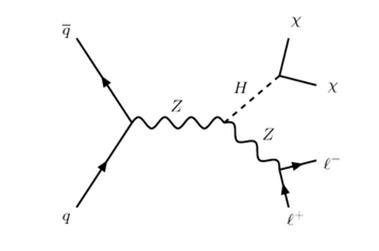
\includegraphics[scale=0.7]{HZ.png}
		\caption{Feynman diagram showing the associated production of Higgs}
		\label{HZ}
	\end{center}
\end{figure}

The background processes are $ZZ\rightarrow ll\nu\nu$, $WZ\rightarrow lll\nu$,$WW\rightarrow l\nu l\nu$, $Z+$jets and $W+$jets. The dominant source of background is the $ZZ \rightarrow ll\nu\nu$ process, contributing $\approx 60 \%$ of the background. 
\begin{figure}[H]
	\begin{center}
		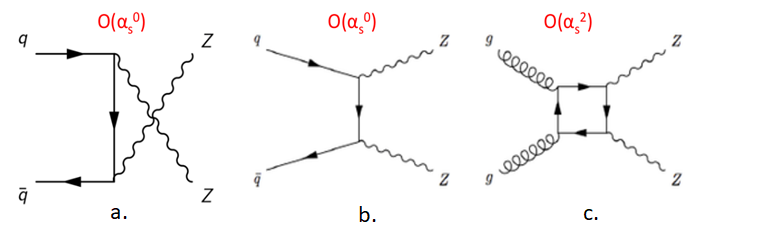
\includegraphics[scale=0.5]{ZZ.png}
		\caption{Feynman Diagram showing $ZZ$ Production \\ a. \& b. $q\bar{q}\rightarrow ZZ$ \hspace{2 cm} c. $gg\rightarrow ZZ$}
		\label{ZZdiag}
	\end{center}
\end{figure}
A precise estimate of this process, along with the uncertainty associated with it, is crucial. In current analyses, this is determined using simulation, with an uncertainty of $\approx 10\%$ \cite{ZH_ATLAS}.

One method of estimating this contribution is to look at $ZZ\rightarrow llll$. However, this suffers from the low branching fraction of $Z\rightarrow ll$, at $\approx 0.46 \%$ \footnote{The branching fraction of $Z$ to any one flavor of lepton is $\approx 3.4\%$, and to neutrinos is $\approx 20\%$.}, and is thus statistically limited.

In similar vein to a earlier analysis that used $\gamma+$jets to calibrate $Z+$jets background \cite{gammajet}, in the $p_T(\gamma) \gg M_Z$ region, the \Zgam process should be kinematically similar to \ZZ as the mass of the $Z$ boson is negligible. Figures \ref{ZZdiag} and \ref{Zgdiag} show the leading order Feynman diagrams for the production of $ZZ$ and $Z+\gamma$ respectively. The diagrams for $q\bar{q}$ and $gg$ (a. b. and c.)are similar. In addition to having a higher $BR*\sigma$ as compared to \ZZ, the \Zgam signal is also very pure. Thus, it should be possible to use \Zgam data to estimate \ZZ contribution to the background, and obtain a more accurate prediction.
\begin{figure}[h]
	\begin{center}
		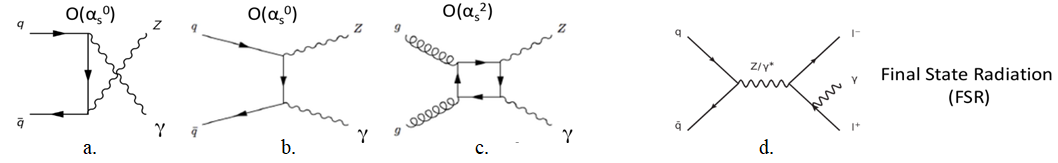
\includegraphics[width=\linewidth]{Zg.png}
		\captionsetup{justification=centering}
		\caption{Feynman Diagram showing $Z+\gamma$ Production\hfill \\ a. \& b. $q\bar{q}\rightarrow Z+\gamma$ \hfill c. $gg\rightarrow Z+\gamma$ \hfill d. Final State Radiation (FSR)}
		\label{Zgdiag}
	\end{center}
\end{figure}

\section{Approach}
Following the method defined in the Ref \cite{gammajet}, we define a variable $R(p_T)$ to be the ratio of the cross sections of \ZZ to \Zgam as a function of $p_T$.
\begin{equation}
	R(p_{T}) = \frac{\sigma_{ZZ}(p_{T})}{\sigma_{Z\gamma}(p_T)}
\end{equation}
With the two processes being kinematically similar at high $p_T$, $R$ depends on the coupling of the $Z$ and $\gamma$ to quarks. It should approach some value asymptotically.

The photon - quark and $Z$ boson - quark couplings in the Standard Model are given by,
\begin{equation}
	-ieQ_q\gamma^{\mu} \hspace{1 cm} \text{and} \hspace{1 cm}\frac{-ie}{2 \sin\theta_W \cos\theta_W}\gamma^{\mu}(v_q - a_q\gamma_5)
\end{equation}
respectively, where $Q_q,v_q$ and $a_q$ are respectively the electric, vector and axial neutral weak couplings of the quarks, and $\theta_W$ is the weak mixing angle. The cross sections are dependent on the matrix elements squared, which contain factors of $Q_q^2$ for $\gamma$, or $(v_q^2 + a_q^2)/4\sin^2 \theta_W \cos^2 \theta_W$ for $Z$. There is a contribution due to the $Z$ mass which appears in the internal propagators and phase space integration. This contribution becomes less important in the $p_T(\gamma)\gg M_Z$ region.

Thus, in the high $p_T$ region, the $Z$ and $\gamma$ cross sections would be in the ratio
\begin{equation}
	R_q = \frac{v_q^2 + a_q^2}{4\sin^2 \theta_W \cos^2 \theta_W * Q_q^2}.
\end{equation} 

Considering the contributions from both $u$ and $d$ flavor quarks,
\begin{equation}
	R = \frac{Z_u \left\langle u \right\rangle + Z_d \left\langle d\right\rangle}{\gamma_u \left\langle u\right\rangle + \gamma_d \left\langle d\right\rangle}
\end{equation}
Substituting $\sin^2 \theta_W = 0.2315$, at moderate $p_T$ values, $R \approx 1.4$\footnote{Equations (3) and (4), as well as the value of $R$ are taken from Ref \cite{gammajet}}.

\begin{figure}[H]
	\centering
		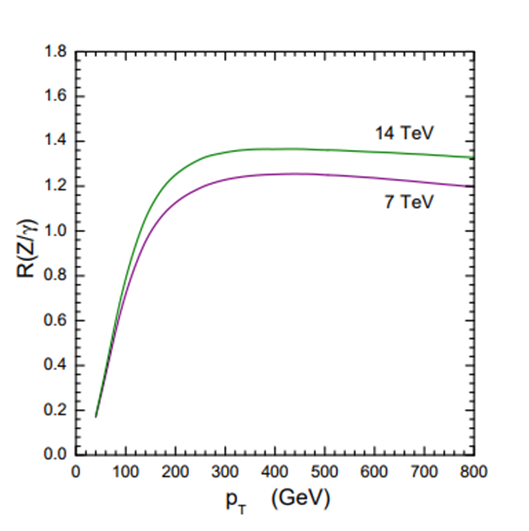
\includegraphics[scale=0.5]{paper_Rplot.png}
		\caption{Ratio of the $Z$ and $\gamma$ $p_T$ distributions \cite{gammajet}}
\end{figure}
This ratio R can be used as is for \ZZ and \Zgam, as the contribution from the $Z\rightarrow ll$ is identically multiplied into the numerator as well as the denominator, and thus cancels out.

\subsection*{MCFM cross sections}
A Monte Carlo program, MCFM v8.0 \cite{MCFM} at NLO, in this case, is used to generate cross sections of \ZZ and \Zgam processes, with a selection of generator level cuts. The samples are generated with cuts on $E_{T,min}^{miss}$ for the $ZZ$ process $p_{T,min}(\gamma)$ for the $Z+\gamma$ process. A ratio of these cross sections is taken to obtain the $R$ curve as a function of $p_T$. The uncertainty on $R$ is calculated by varying several parameters at the generator level, such as the renormalization and factorization scales, the PDF sets used, photon fragmentation, etc. Effects of applying lepton cuts on the cross sections as well as the ratio, and the contributions of the $q \bar{q}$ and $gg$ processes are also studied.

However, the MCFM generator only produces $Z\rightarrow ee$ instead of $Z\rightarrow ll$. Thus, this branching ratio needs to be accounted for to obtain the value of $R$.
\begin{equation}\label{eq:R_inc}
	R_{inc} = R * \frac{BR(Z\rightarrow ee)}{BR(Z \rightarrow ee)*BR(Z\rightarrow \nu\nu)*2}
\end{equation}

\subsection*{Monte Carlo samples - DxAODs}
MCFM gives differential cross sections. Thus the next step is to run the analysis on generated Monte Carlo samples that give event information. The cuts on the leptons, such at $p_T$, $\eta$ and the di-lepton mass window are applied consistently to both.

Monte Carlo events samples are generated using the ATHENA framework \cite{ATHENA}, at NLO. They are then converted to TRUTH3 DxAOD format for analysis. The analysis is implemented using a Python script.

Only events that pass all the cuts are kept. The fraction of such events is multiplied with the total cross section of the generated sample to obtain the cross section corresponding to the event subset we are interested in.
\begin{equation}
	\frac{passed\ events}{total\ events}*\sigma_{xAOD}
\end{equation}
where
\begin{center}
\label{eq:xAOD_xsec_frac}
$\sigma_{xAOD} = 923.18 \text{ fb}$
\end{center}

It is necessary to check the consistency for each of the processes, before proceeding to calculate the ratio $R$.

\section{Generator Parameters}
The samples are generated using MCFM v8.0 for the following data points\footnote{MCFM does not generate $Z\rightarrow ll$ but $Z\rightarrow ee$. As electrons and muons have similar properties with the exception of mass, simply the branching fraction of $Z\rightarrow ee$ must be accounted for at a later stage.}
\begin{align*}
	\text{For } ZZ \rightarrow ee\nu\nu &: E_T^{miss} > \{50,75,100,125,150,200,250,300,400,500\}\text{ GeV} \\
	\text{For } Z(\rightarrow ee)+\gamma &: p_T(\gamma) > \{50,75,100,125,150,200,250,300,400,500\}\text{ GeV}
\end{align*}

Table \ref{table:default} lists the generator level settings used for the $ZZ$ and $Z+\gamma$ processes. All lepton cuts are consistent with the ones used in the ATLAS Z+MET analysis.
\begin{table}[H]
\begin{center}
	\begin{tabular}{|c|c|c|}
	\hline
	\textbf{Cuts} &$ZZ \rightarrow ee\nu\nu$ & $Z(\rightarrow ee)+\gamma$\\
	\hline
	Process ID & 87 & 300\\
	$M_{ee}$ & $81 < M_{ee} < 101$ GeV & $81 < M_{ee} < 101$ GeV\\
	$M_{\nu\nu}$ & $81 < M_{\nu\nu} < 101$ GeV& -\\
	Order & NLO & NLO\\
	PDFset & CT14 & CT14\\
	$p_T^{\text{lead}}(e)$ & $> 30$ GeV & $> 30$ GeV\\
	$\eta^{lead}(e)$ & $< 2.5$ & $< 2.5$\\
	$p_T^{\text{sublead}}(e)$ & $> 20$ GeV & $> 20$ GeV\\
	$\eta^{sublead}(e)$ & $< 2.5$ & $< 2.5$\\
	$\Delta R(\gamma,e)$ & - & 0.7\\
	Renormalization scale & $91.187$ GeV & $91.187$ GeV $(M_{Z})$\\
	Factorization scale & $91.187$ GeV & $91.187$ GeV $(M_{Z})$\\
	\hline
	\end{tabular}
	\caption{Settings in input.DAT for MCFM}
	\label{table:default}
	\end{center}
\end{table}

The constraint on $M_{ee}$ in the case of $Z+\gamma$ suppresses the FSR process by ensuring that the lepton pair are from a $Z$ decay only.
\newpage
\section{Results}

\subsection*{Uncertainties with MCFM}
\label{subsec:MCFM_unc}
\addcontentsline{toc}{subsection}{\nameref{subsec:MCFM_unc}}
\setcounter{subsection}{1}
Upon running the steering file with the parameters described above, the cross sections shown in Figure \ref{xsecs} are obtained. Throughout this analysis, this sample is the reference.

\begin{figure}[H]
\centering
	\begin{subfigure}{0.49\textwidth}
		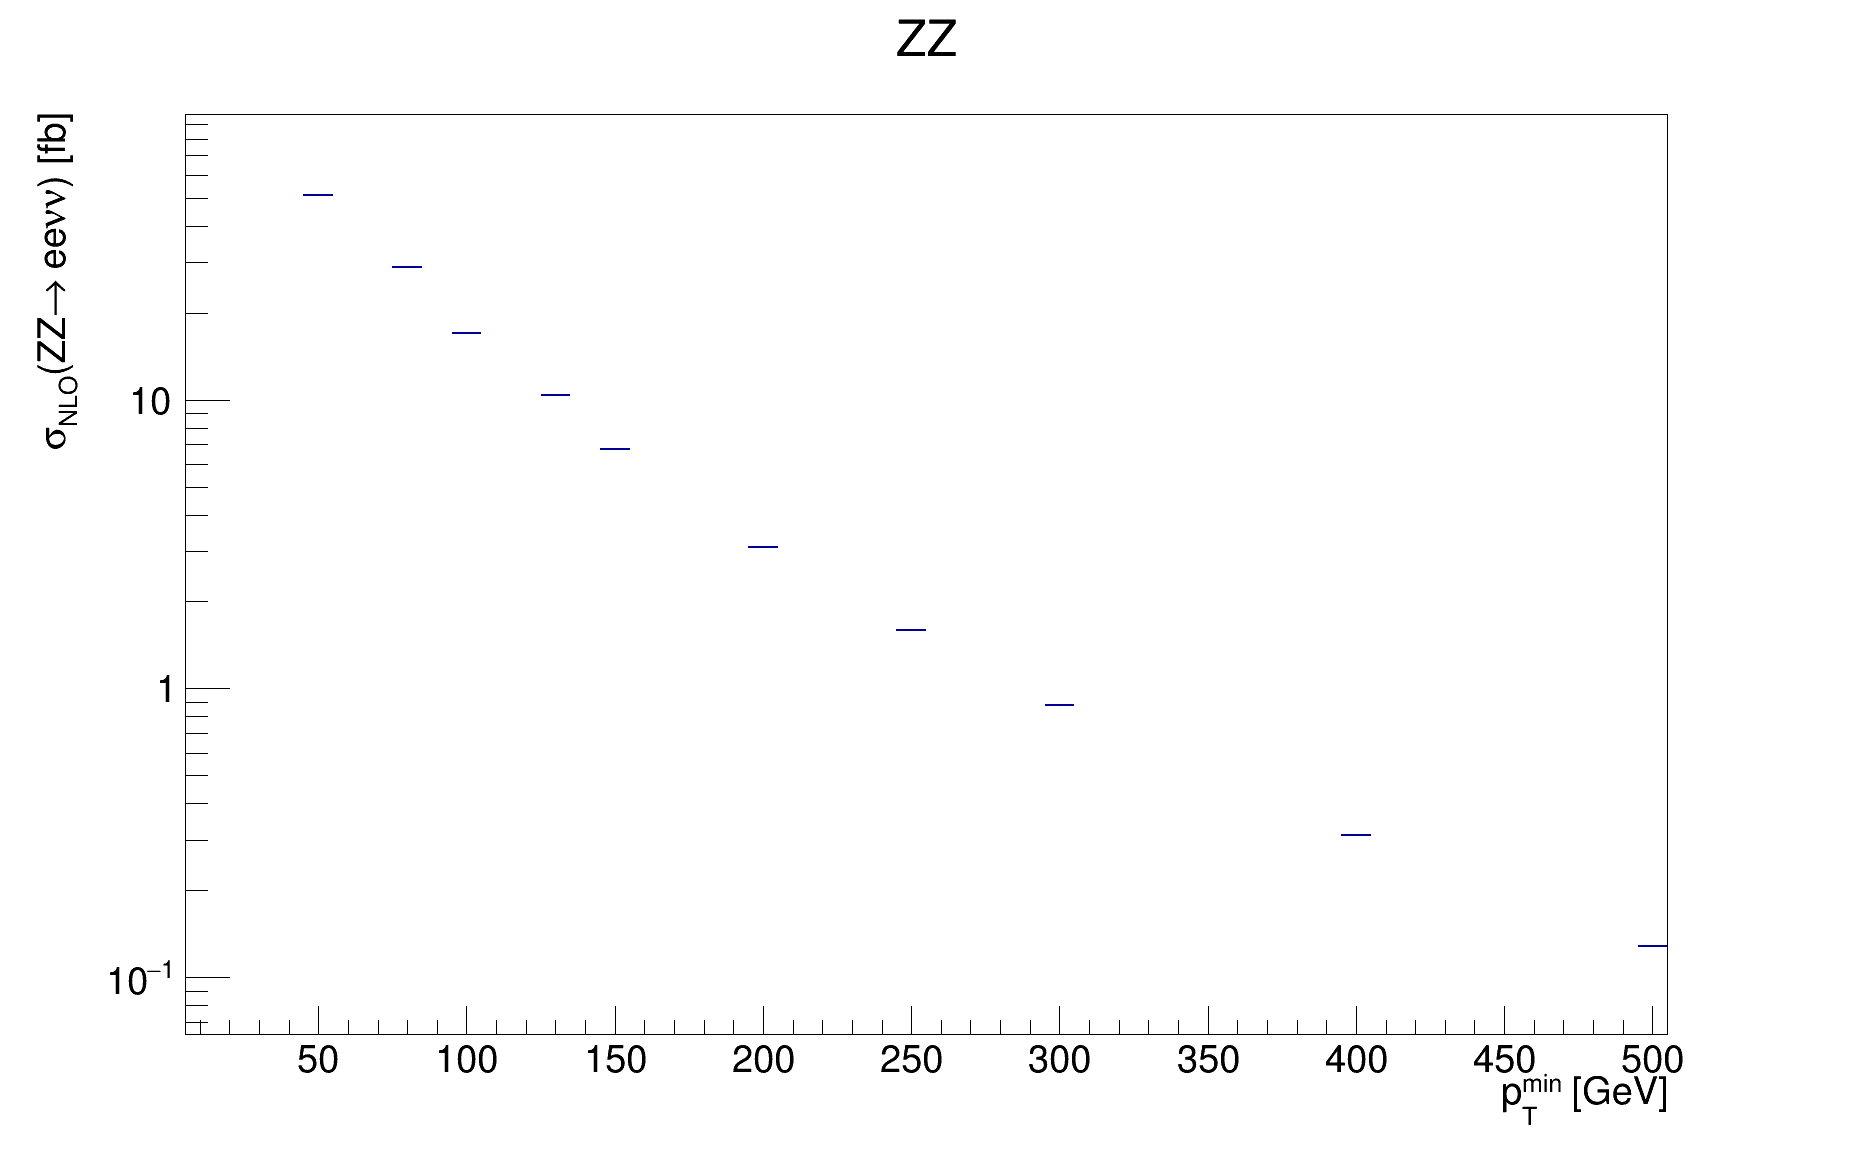
\includegraphics[width=\linewidth]{ZZ_xsec.png}
		\caption{$ZZ\rightarrow ee$ cross section}
	\end{subfigure}	
	\begin{subfigure}{0.49\textwidth}
		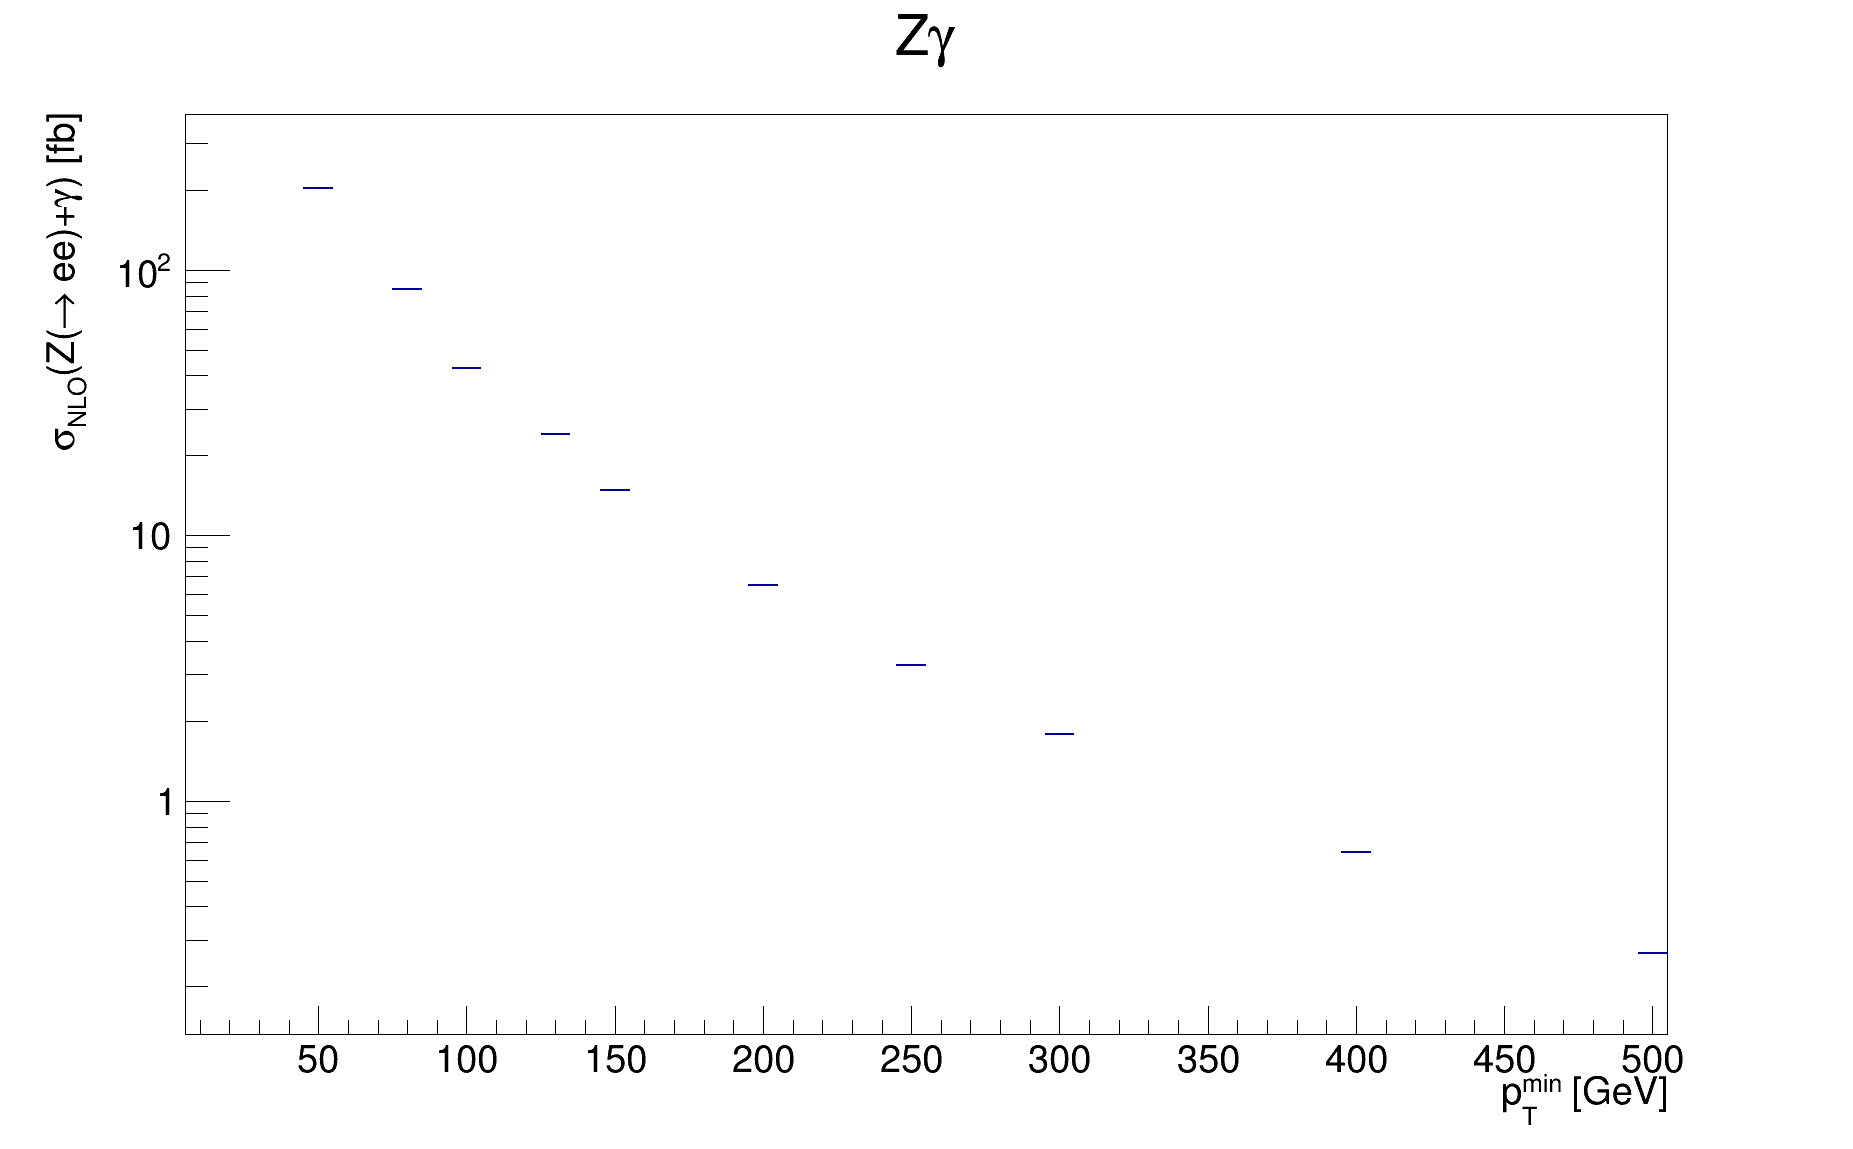
\includegraphics[width=\linewidth]{Zg_xsec.png}
		\caption{$Z(\rightarrow ee)+\gamma$ cross section}
	\end{subfigure}
	
	\caption{Cross sections of $ZZ$ and $Z+\gamma$ processes with the cuts as in Table 1. The Y axis is in $\log_{10}$ scale.}
	\label{xsecs}
\end{figure}

The resulting ratio is shown in Figure \ref{fig:Rcurve}
\begin{figure}[H]
	\centering
	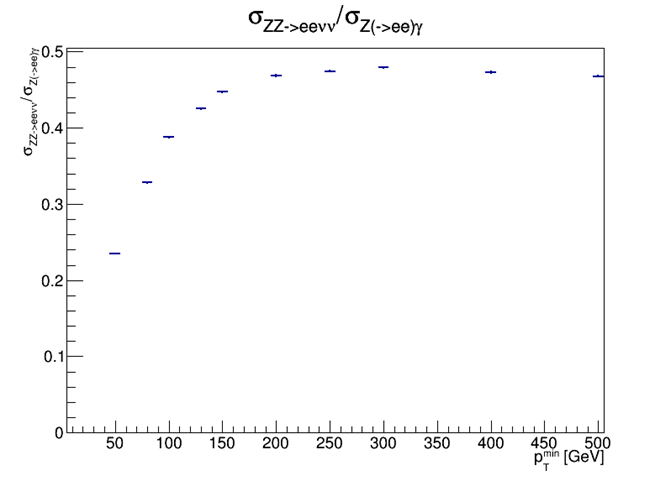
\includegraphics[scale=0.7]{Ratio_default.png}
	\caption{$R$ curve as a function of $p_T$}
	\label{fig:Rcurve}
\end{figure}
The $R$ value is observed to increase from $\approx 0.24$ at 50 GeV to $\approx 0.47$ at high $p_T$, where it is constant. When the branching ratio is accounted for as show in Equation \ref{eq:R_inc}, the resulting $R(p_T)$ curve is shown in Figure \ref{fig:RcurveBR}, increasing from $\approx 0.61$ at 50 GeV to $\approx 1.2$ at high $p_T$.
\begin{figure}[H]
	\centering
	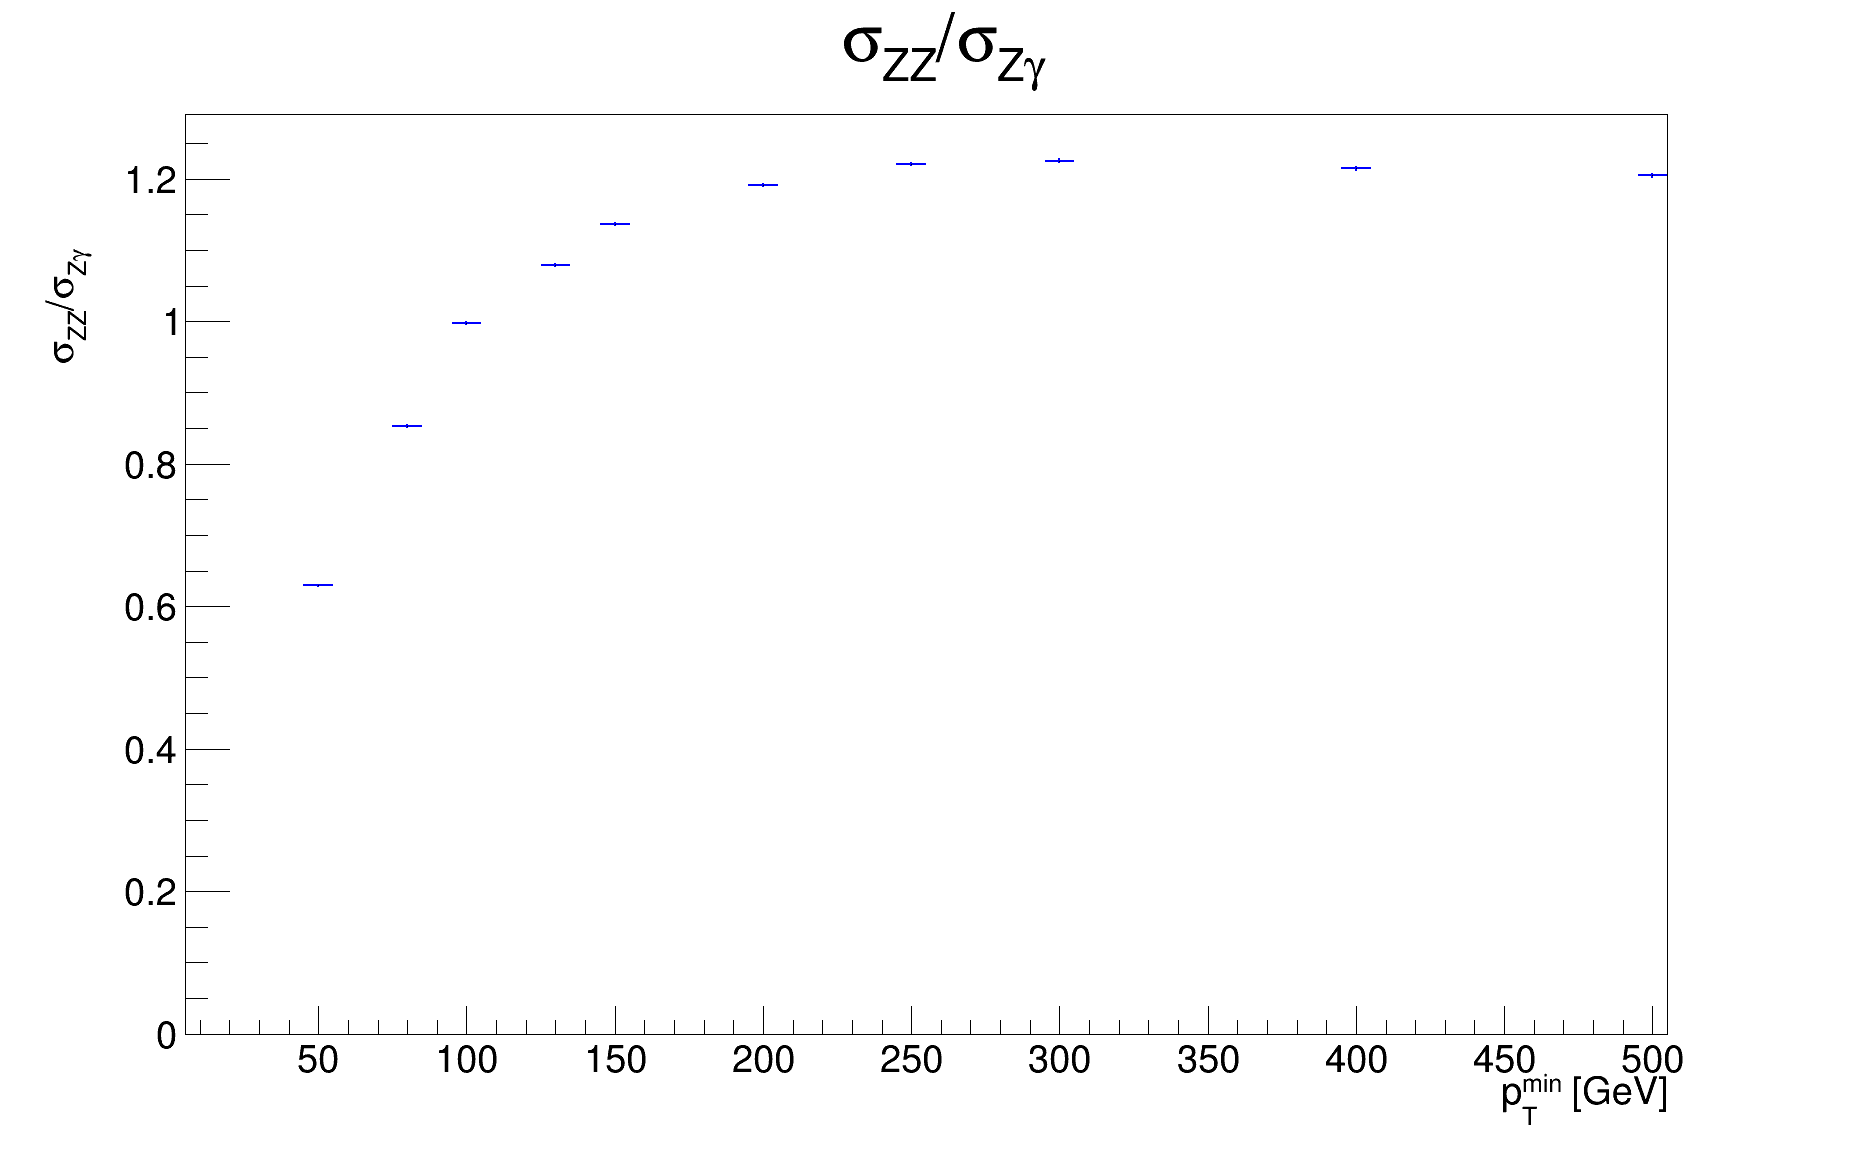
\includegraphics[width = 0.8\textwidth]{Ratio_with_BR.png}
	\caption{$R$ curve as a function of $p_T$, accounting for the $Z\rightarrow ee$ and $Z\rightarrow \nu\nu$ branching ratios.}
	\label{fig:RcurveBR}
\end{figure}

Figure \ref{fig:R_gg_qq} shows the $R$ curve obtained from the $gg$ process, as well as the $R$ curve from the $q\bar{q}$ and $qg$ processes.
\begin{figure}[H]
\centering
	\begin{subfigure}{0.49\textwidth}
		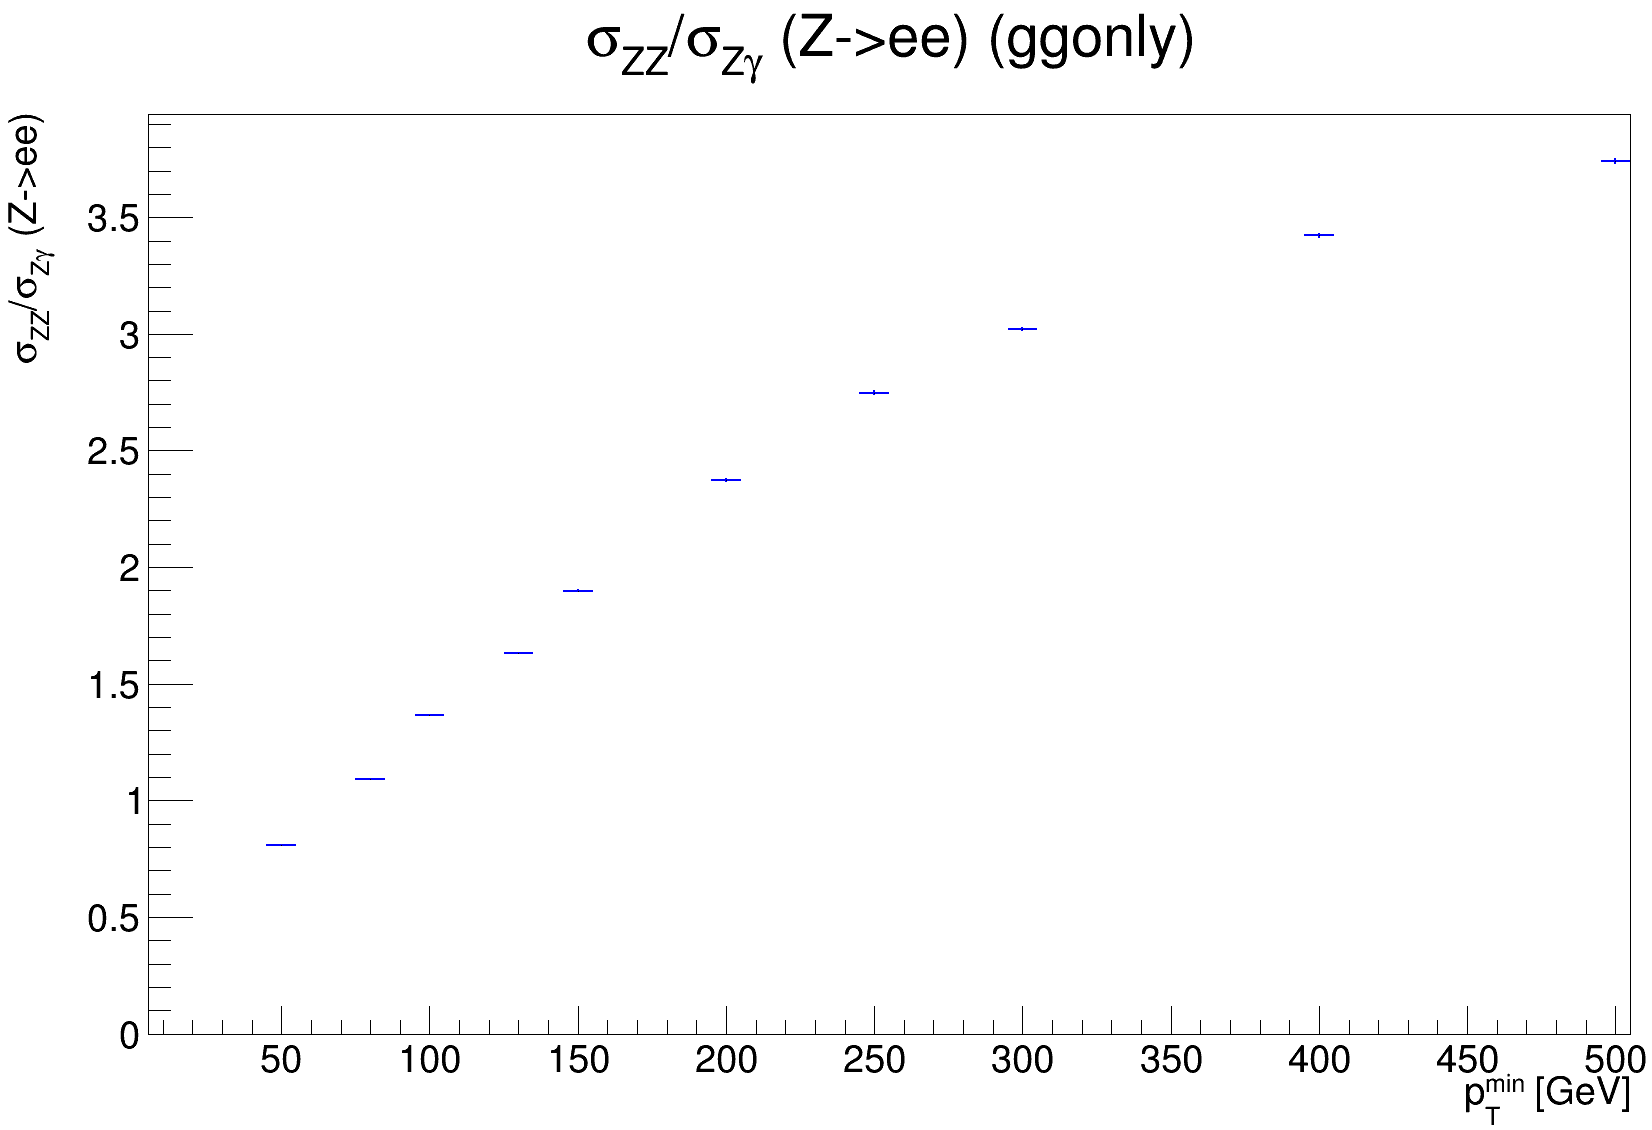
\includegraphics[width=\linewidth]{R_ggonly.png}
		\caption{$R_{gg}$ curve from $gg$ subprocess only}
	\end{subfigure}
	\begin{subfigure}{0.49\textwidth}
		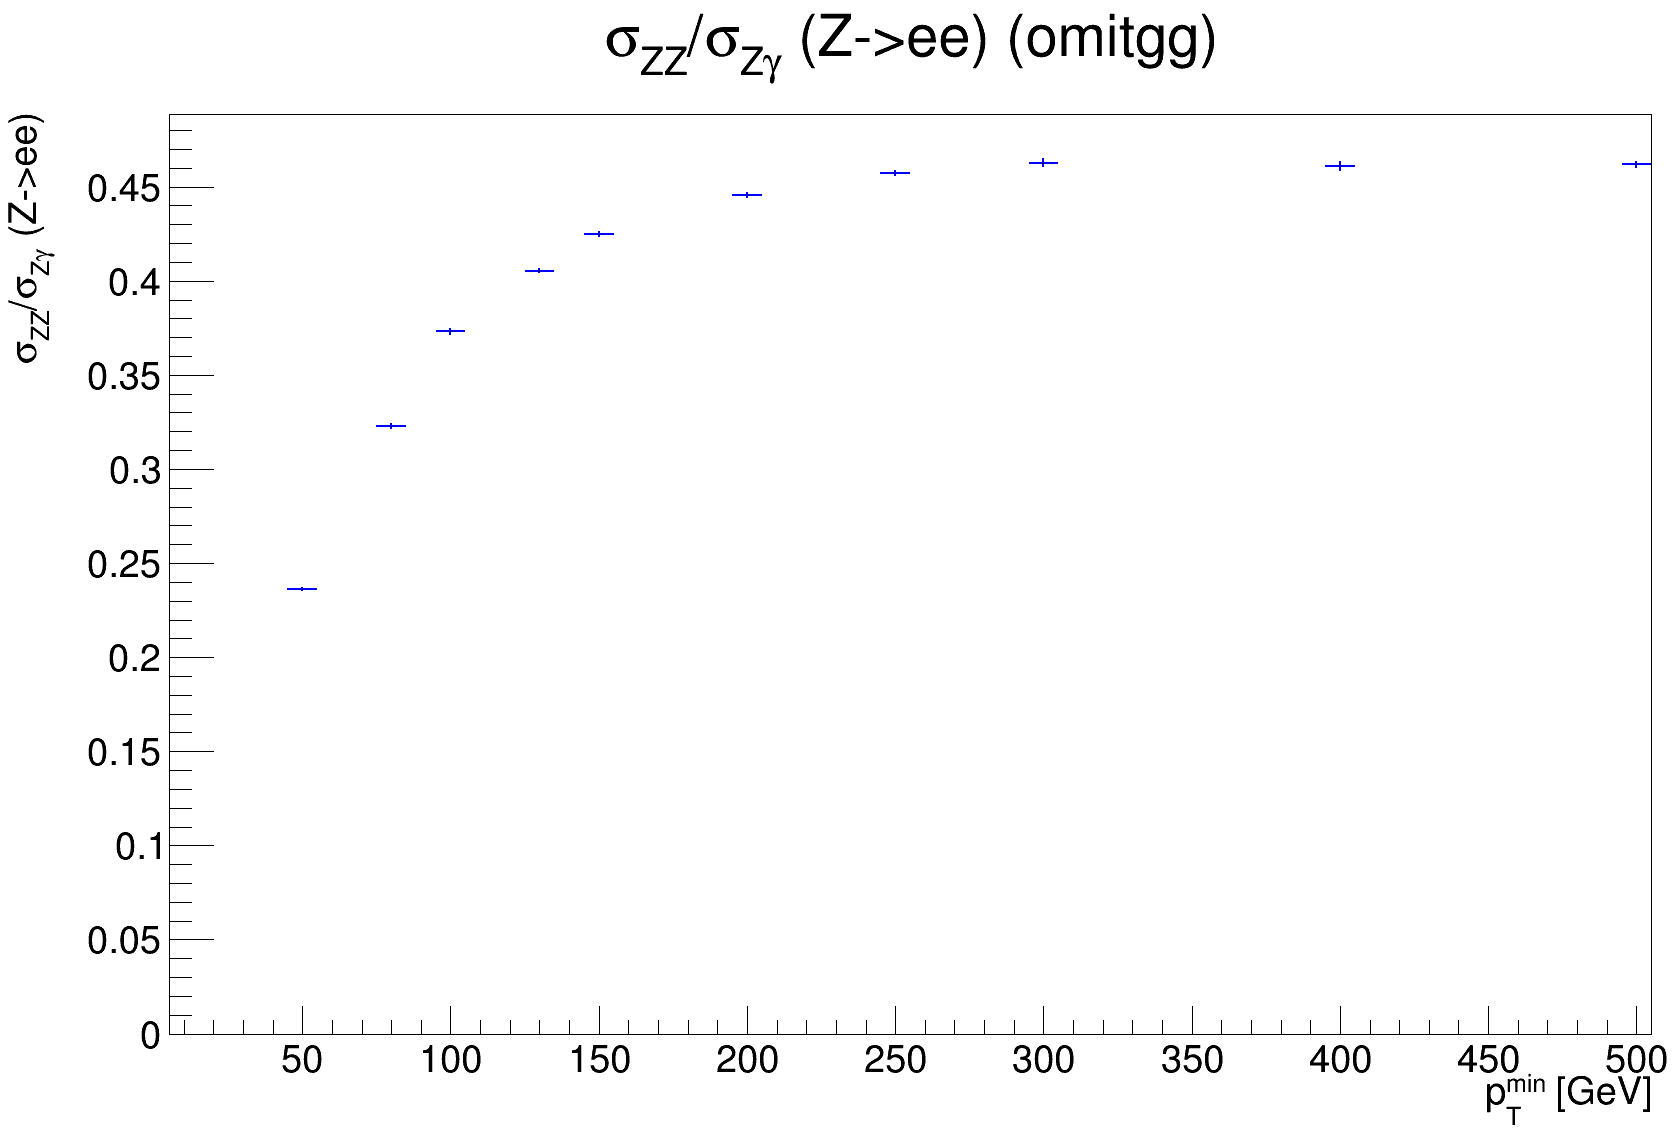
\includegraphics[width=\linewidth]{R_omitgg.png}
		\caption{$R_{q\bar{q}/qg}$ curve from $q\bar{q}$ and $qg$ subprocesses}
	\end{subfigure}	
\caption{The ratio $R(p_T)$ from the contributing quark and gluon processes.}
\label{fig:R_gg_qq}
\end{figure}

\subsubsection{Effect of Lepton Cuts}
To check the effects of lepton cuts on the ratio, samples with similar parameters as those in Table \ref{table:default} are generated. However, we relax the cuts on leptons. Both the leading and subleading lepton should have $p_T > 5$ GeV, and $\eta <$ 10. In the lower $p_T$ regions, the cross section falls by nearly half in both processes. However, the ratio is not affected very much, as seen in Figure \ref{fig:lepcut}.
\begin{figure}[H]
\centering
	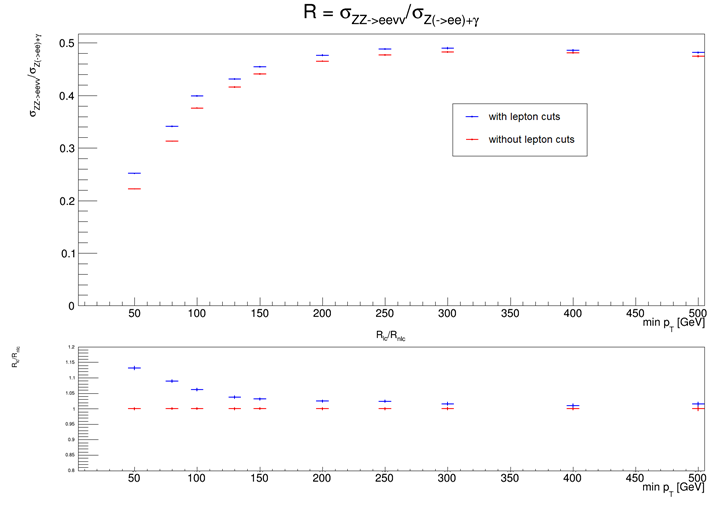
\includegraphics[width = 0.7\linewidth]{lep_cuts.png}
	\caption{Comparison of reference $R$ curve to $R$ curve without lepton cuts}
	\label{fig:lepcut}
\end{figure}
The $R$ curves differ by $\approx 4\%$ at high $p_T$, and $\approx 7\%$ at 100 GeV. This is not an uncertainty, but the effect of applying lepton cuts on each of the processes.

\subsubsection{Scale Variation}
The Renormalization and Factorization scales are arbitrary parameters that address the UV and IR divergences respectively that arise while calculating cross sections. They are important when considering higher order effects in QCD. To obtain the uncertainties associated to these scales, the Renormalization ($\mu_R$) and Factorization ($\mu_F$) scales are each varied by a factor of 2 in either direction from the central value, $M_Z = 91.187$ GeV, to obtain the uncertainty as shown in Figure \ref{fig:scalecompare}.
\begin{figure}[H]
\centering
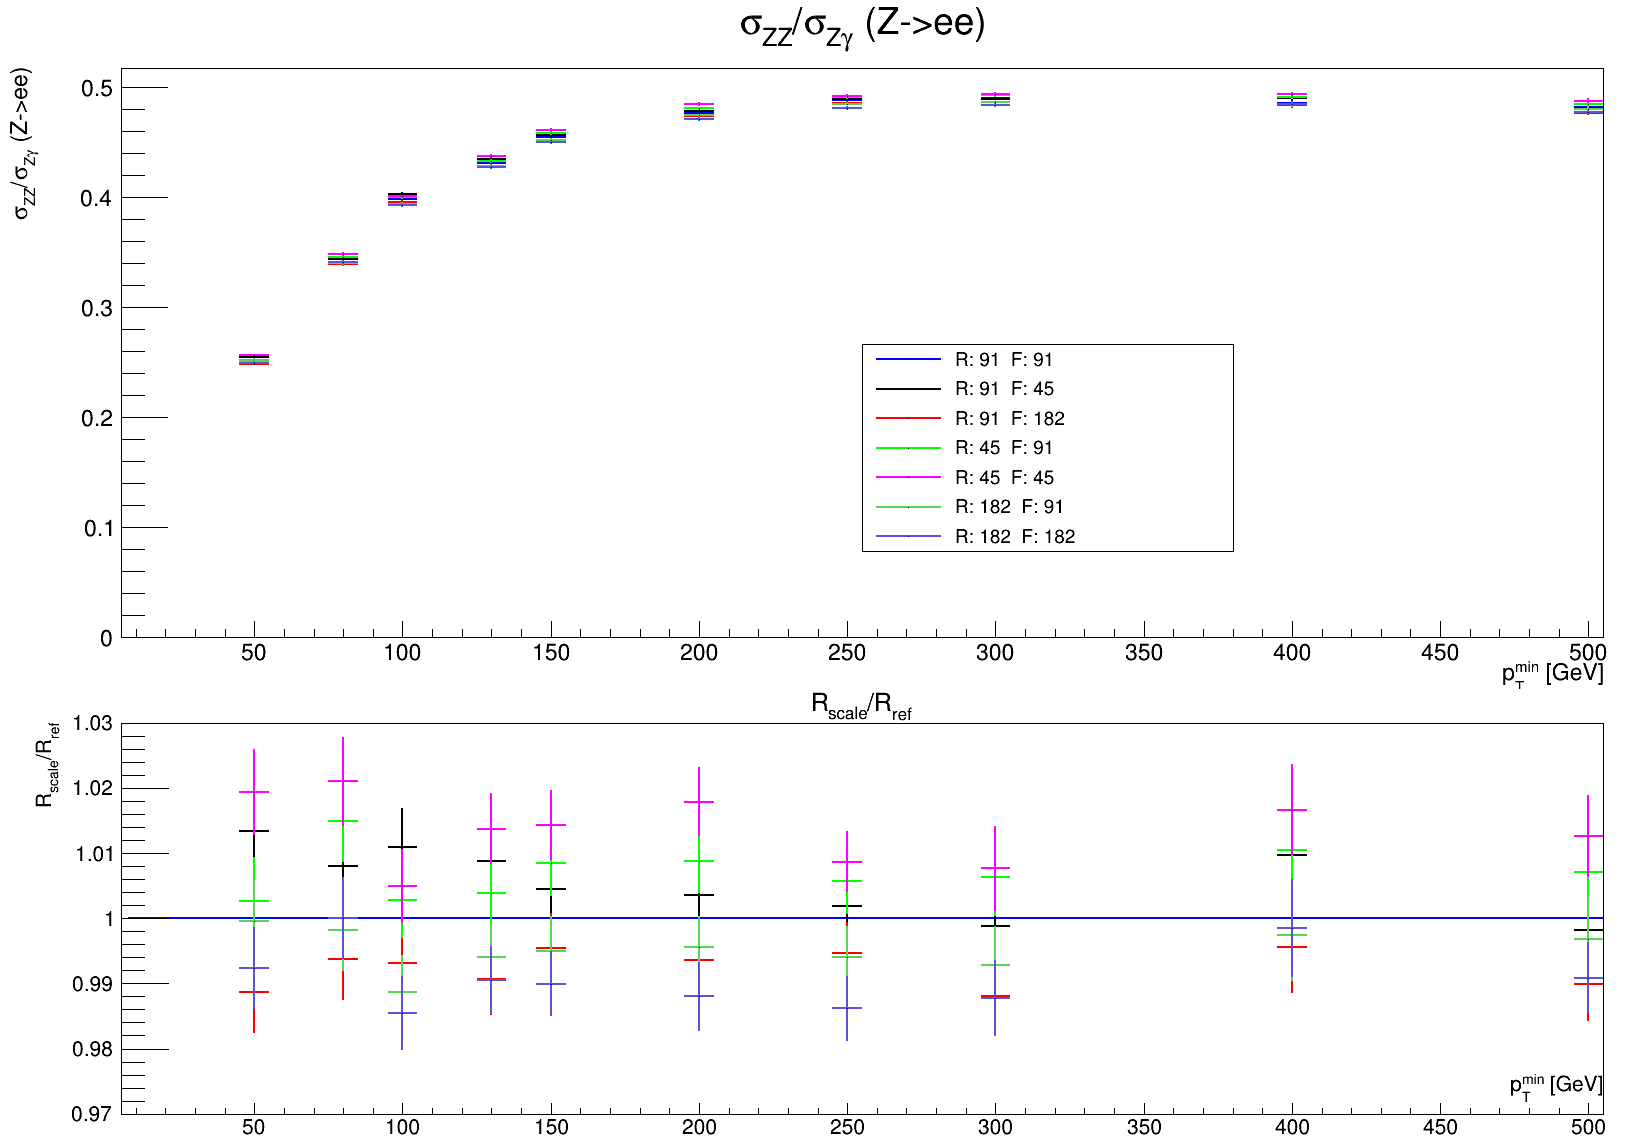
\includegraphics[width=0.8\linewidth]{scale/nlo_scale_overlay.png}
\caption{The ratio $R(p_T)$ for various choices for $\mu_R$ (R) and $\mu_F$ (F). The bottom panel shows the relative - with respect to the reference (R: 91, F: 91) for each scale. The uncertainties are statistical}
\label{fig:scalecompare}
\end{figure}
The uncertainty due to the variation of scales around $R = 0.398$ is $\pm \approx 2\%$ for all $p_T$.

Looking at the the contribution of the $gg$ subprocess separately from the $q\bar{q}$ and $qg$ subprocesses, the result is shown in Figure \ref{scale}.
\begin{figure}[H]
\centering
	\begin{subfigure}{0.49\textwidth}
		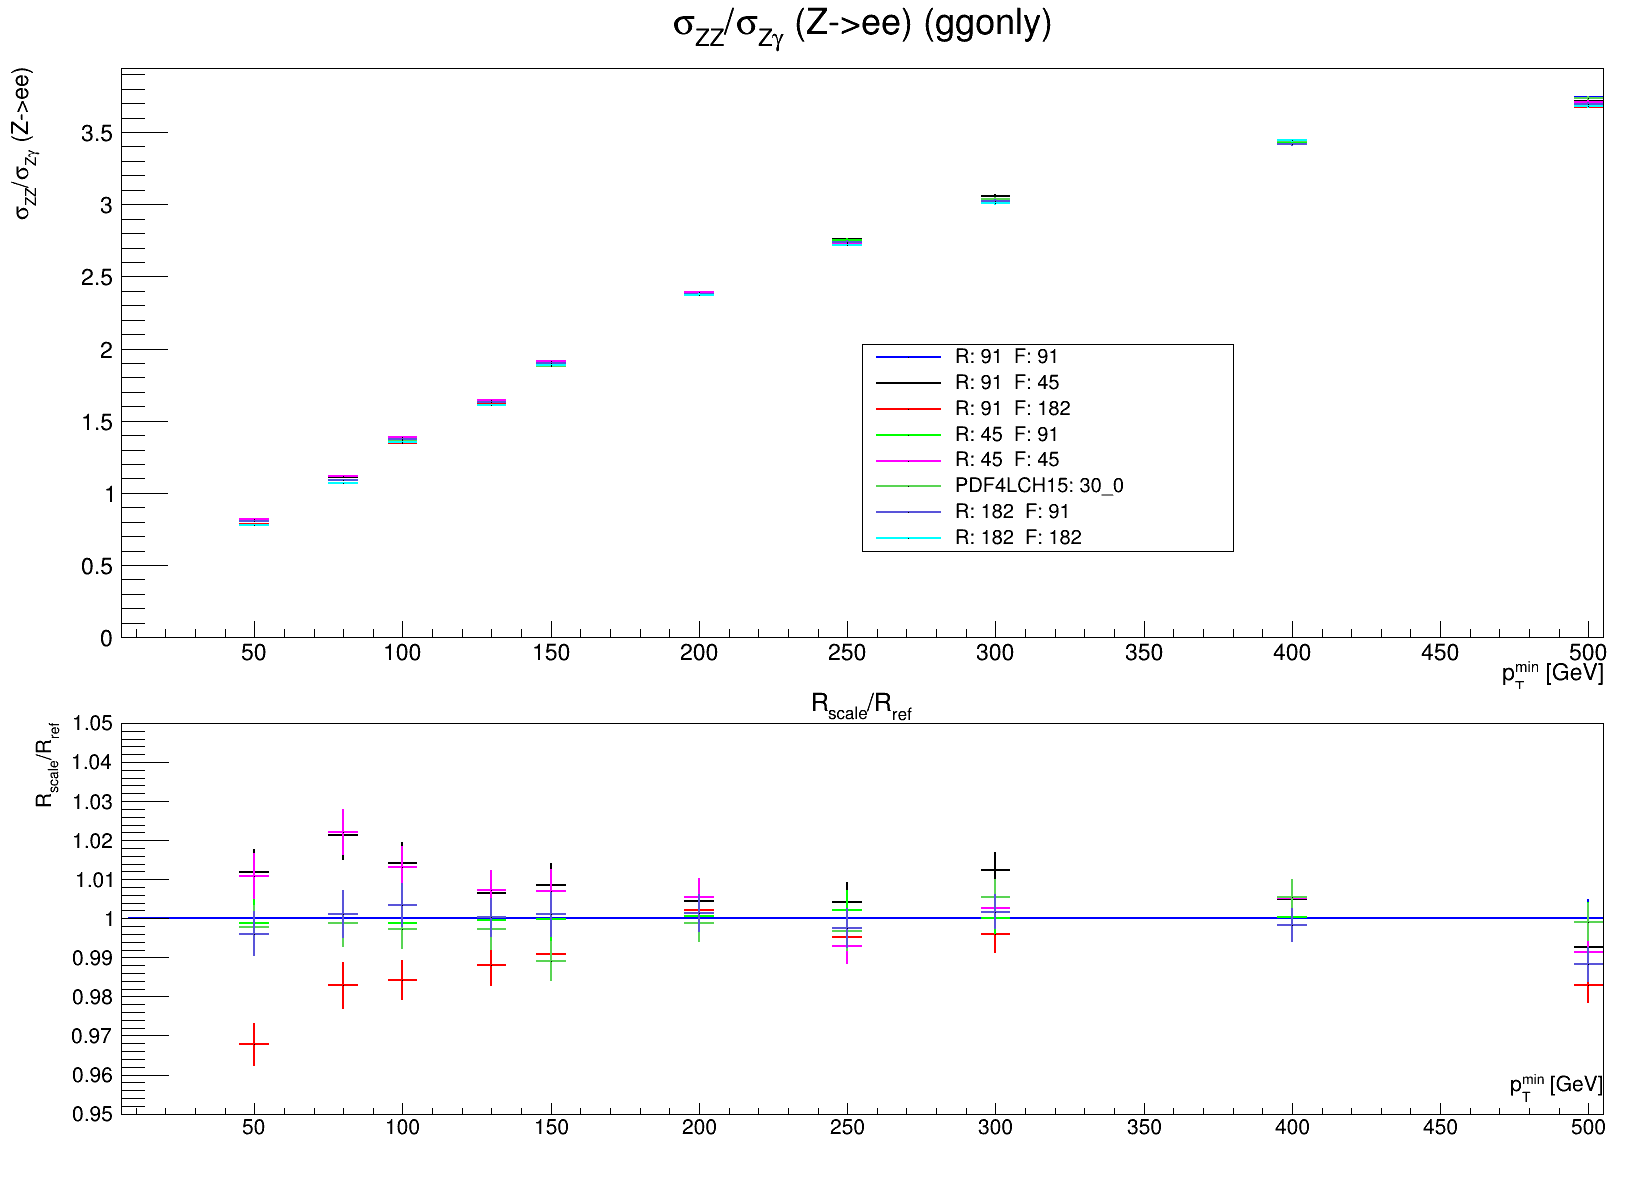
\includegraphics[width=\linewidth]{scale/ggonly_nlo_scale_overlay.png}
		\caption{$R_{gg}$ curve from $gg$ subprocess only}
	\end{subfigure}
	\begin{subfigure}{0.49\textwidth}
		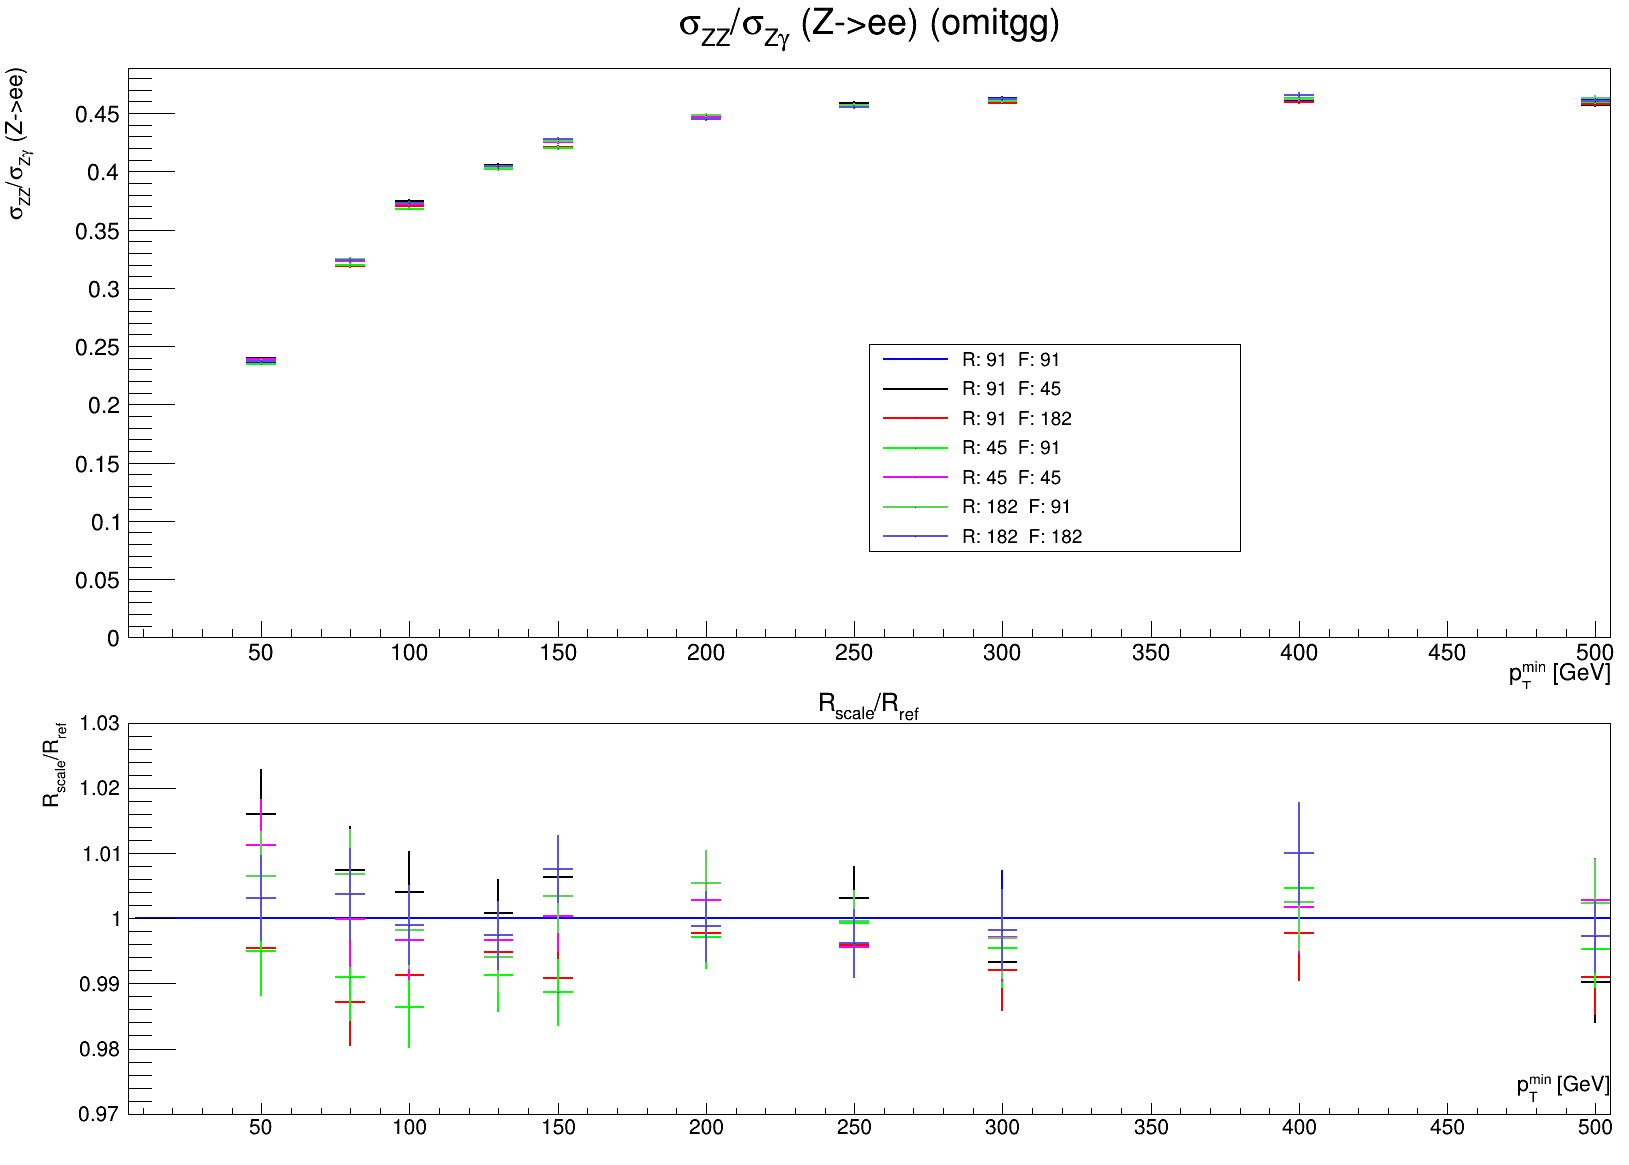
\includegraphics[width=\linewidth]{scale/omitgg_nlo_scale_overlay.png}
		\caption{$R_{q\bar{q}/qg}$ curve from $q\bar{q}$ and $qg$ subprocesses}
	\end{subfigure}	
\caption{The ratio $R(p_T)$ for various choices for $\mu_R$ (R) and $\mu_F$ (F) for the $gg$ and $qg+q\bar{q}$ subprocesses separately. The bottom panel shows the relative difference with respect to the reference (R: 91, F: 91) for each scale. The uncertainties are statistical.}
\label{scale}
\end{figure}
Gluon-gluon processes contribute to 8.6\% of the total cross section for the $ZZ$ process and 2.5\% of the $Z+\gamma$ process. An uncertainty of $\pm \approx 2\%$ around $R_{gg} = 1.37$ at 100 GeV and is $< 4\%$ for all $p_T$. It remains to understand the shape and magnitude of the $R$ curve for $gg$ processes.

\subsubsection{PDF variation}
The PDF set used for reference is the \texttt{CT14}\cite{CT14} PDF set. To study the variation due by varying PDFs, the PDF sets used are \texttt{PDF4LHC15}\cite{PDF4}, constructed from the combination of \texttt{CT14,MMHT14}\cite{MMHT14} and \texttt{NNPDF3.0}\cite{NNPDF3} PDF sets. These sets are provided by LHAPDF6\cite{LHAPDF}. \texttt{PDF4LHC15} gives access to different PDF groups. The group used here is \texttt{PDF4LHC15\_nlo\_30}, consisting of 30 PDF sets. While the most accurate uncertainties are given by \texttt{PDF4LHC15\_nlo\_100} sets, \texttt{PDF4LHC15\_nlo\_30} is used here for a faster, reasonably accurate estimate of the uncertainties.
\begin{figure}[H]
\centering
	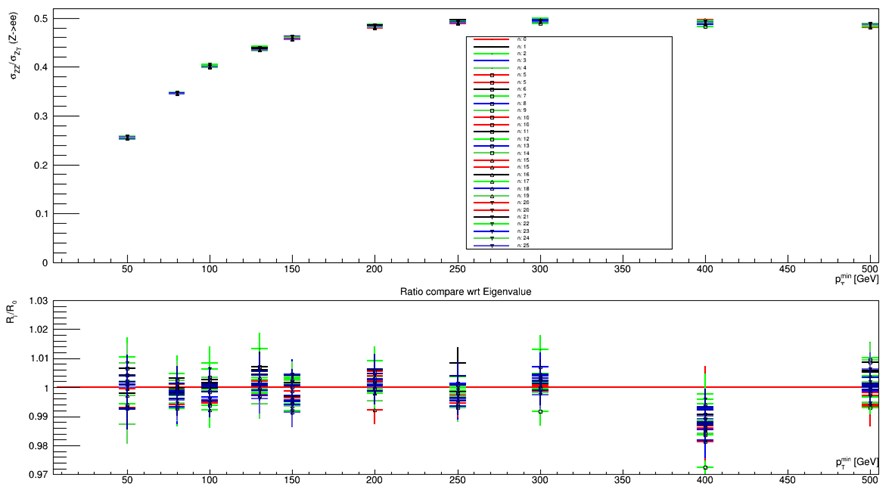
\includegraphics[width = 0.8\linewidth]{PDF4_30_overlay.png}
	\caption{The ratio $R(p_T)$ for each of the 30 PDF sets in \texttt{PDF4LHC15\_nlo\_30}. The bottom plot shows the relative differences of sets 1-30, with respect to set 0 which is taken as the central value.}
	\label{fig:PDF30var}
\end{figure}
\noindent Fig.\ref{fig:PDF30var} shows the comparison of the ratio curves $R(p_T)$ from the 30 member sets of \texttt{PDF4LHC15\_nlo\_30}. To measure the uncertainty due to these 30 sets, the relation as stated in Equation 20 in Ref \cite{PDF4} is used:
\begin{equation}\label{eq:PDFerr}
	\delta^{PDF}\sigma = \sqrt{\sum^{N_{mem}}_{k=1} (\sigma^{(k)} - \sigma^{(0)})^2}
\end{equation}
where $N_{mem}$ is the number of member sets in the group, in this case, 30. The $R$ curve obtained from the \texttt{PDF4LHC15\_nlo\_30} set is compared to the reference curve from \texttt{CT14}, as shown in Figure \ref{pdfcompare}:
\begin{figure}[H]
\centering
	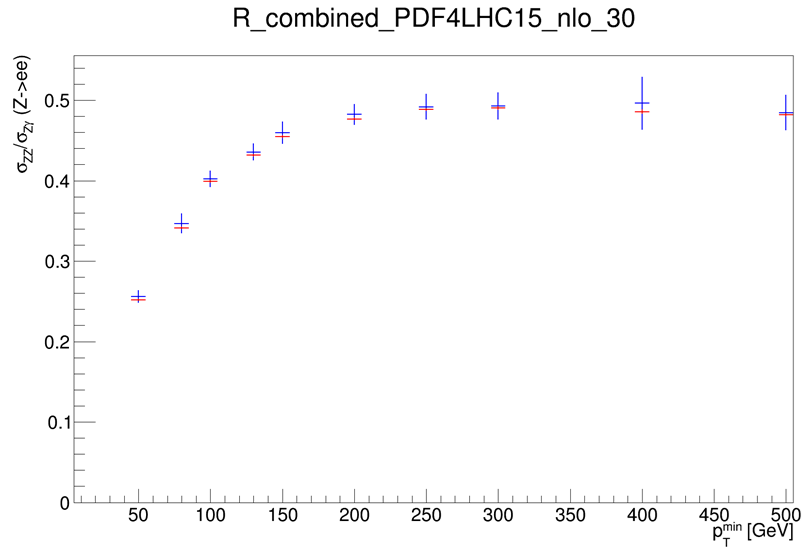
\includegraphics[width = 0.55\linewidth]{PDF4_CT14_comp.png}
	\caption{The ratio $R(p_T)$ of the \texttt{PDF4LHC15\_nlo\_30}, with combined uncertainties as given by Equation \ref{eq:PDFerr}, to the reference constructed from the PDF set \texttt{CT14}}
	\label{fig:PDF4_def_compare}
	\label{pdfcompare}
\end{figure}
\noindent Fig.\ref{fig:PDF4_def_compare} shows a comparison between the central value of the sets in \texttt{PDF4LHC15\_nlo\_30} with the combined uncertainties, and the reference PDF set \texttt{CT14}. The combined uncertainty around $R \approx 0.40$ is $\pm 2.55\%$ at 100 GeV. The PDF sets agree to within the uncertainty bounds. The contributions of the $gg$ subprocess to the cross sections, and the $R_{gg}$ curve are also studied, as shown in Figure \ref{pdfcompare_gg}.
\begin{figure}[H]
\centering
	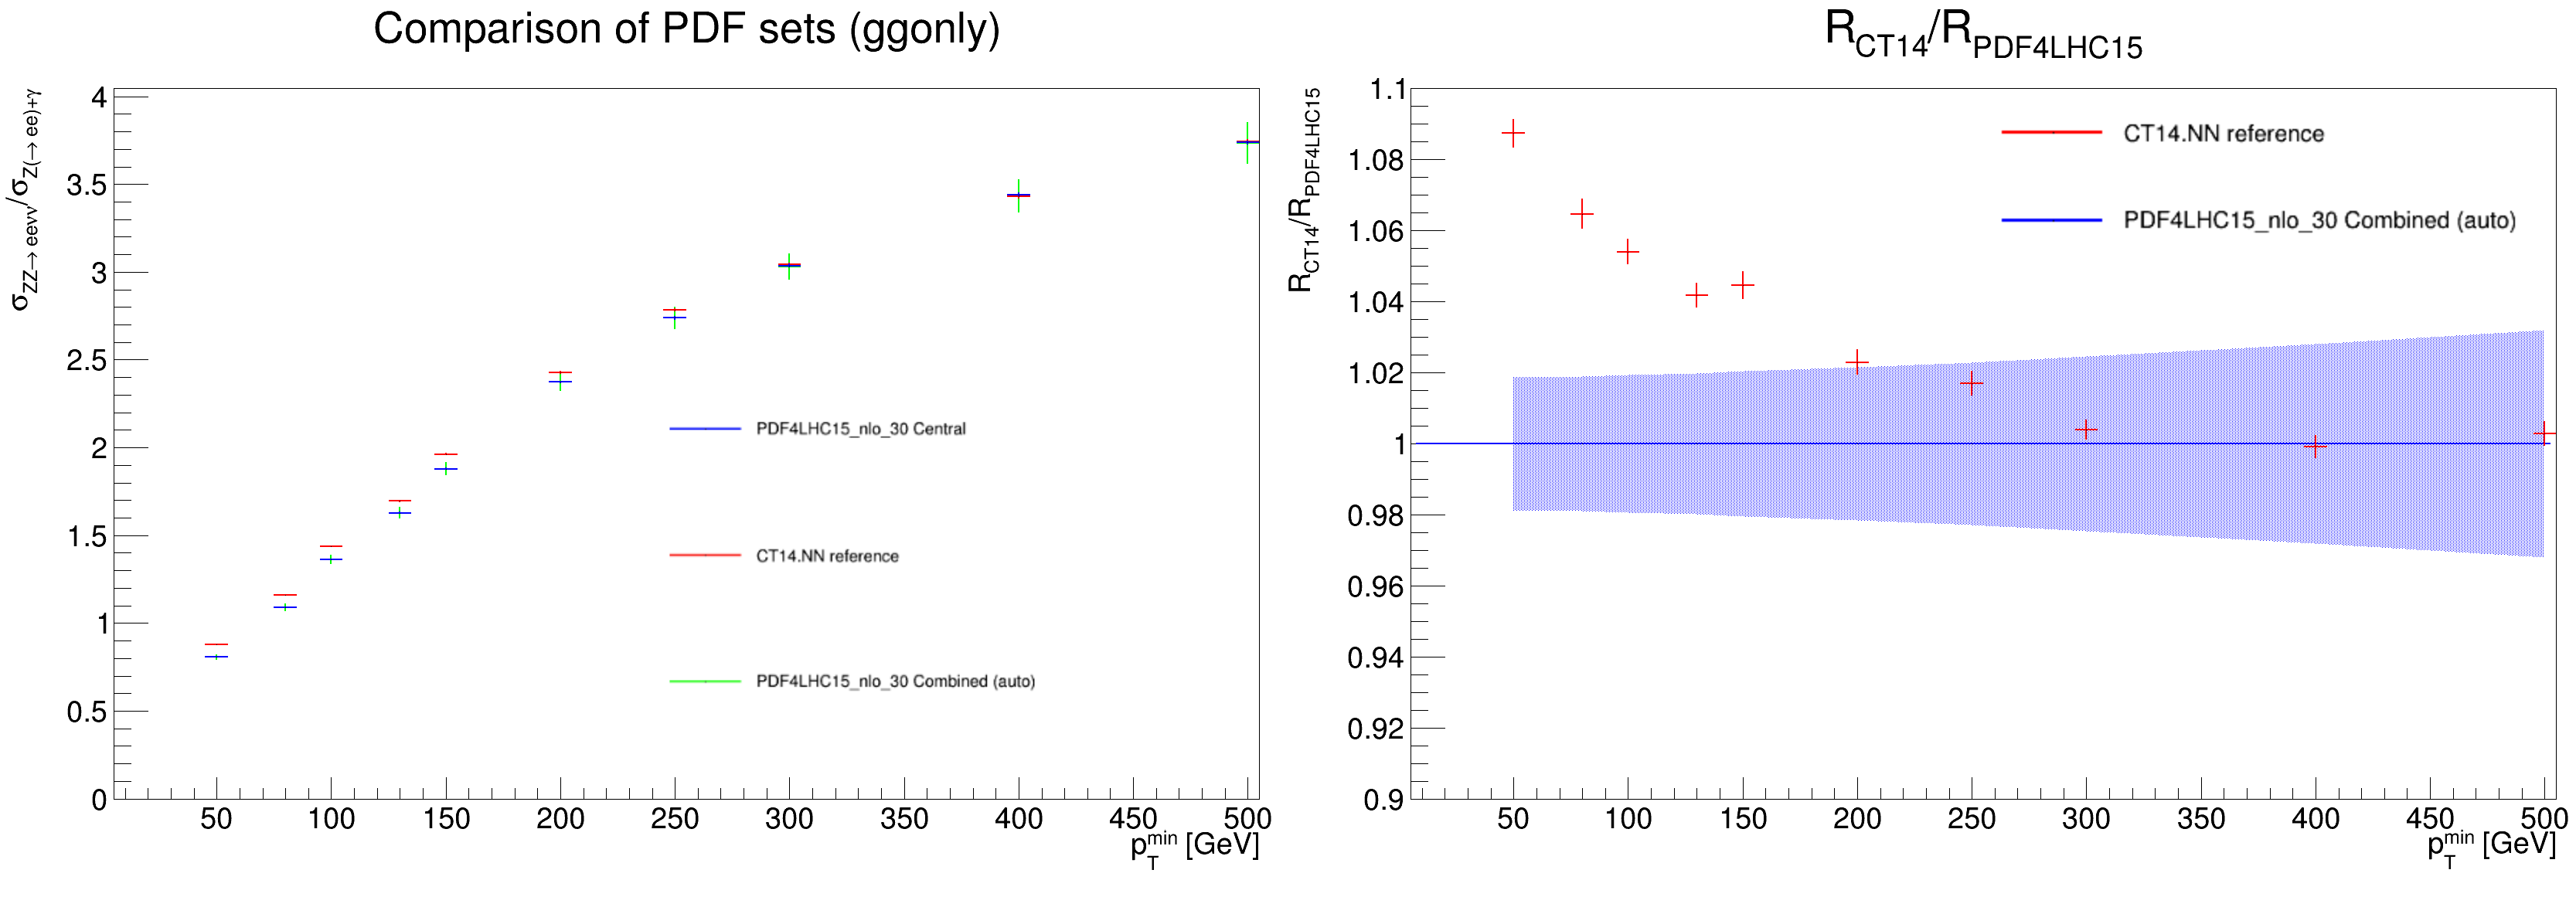
\includegraphics[width=\textwidth]{gg_PDF4.png}
	\caption{$R_{gg}$ curve plotted from only the $gg$ contribution to the cross sections of $ZZ$ and $Z+\gamma$, using the combined uncertainties of \texttt{PDF4LHC15\_nlo\_30} sets. The figure on the right shows the ratio of the \texttt{CT14} set to the \texttt{PDF4LHC15\_nlo\_30} set.}
	\label{pdfcompare_gg}
\end{figure}
The $gg$ contributions differ by a factor of 10. This curve appears to reach an a constant value at a higher $p_T$ value than the ratio curve constructed from the total cross section. The gluon gluon process is of interest, thus it has also been compared to the reference \texttt{CT14} set.

\subsubsection{Photon Fragmentation}
The \Zgam process may contain photons that arise from the hadron showers. It is therefore important to isolate the prompt photon from hadronic activity. This reduces unwanted background from pion decays, or fragmentation processes.

Experimentally, photon isolation is implemented with the following cuts:
\begin{equation}
\sum_{\in R_0} E_T(\text{had}) < \epsilon_h p_T^\gamma \text{\hspace{1cm} or \hspace{1cm}} \sum_{\in R_0} E_T(\text{had}) < E_T^{max}
\end{equation}
\label{eq:photon_isol}
limiting the transverse hadronic energy $E_T(had)$ in a cone of size $R_0 = \sqrt{\Delta\eta^2 + \Delta\phi^2}$ around the photon, to some fraction of the photon $p_T$, or some fixed small cut-off.

The smooth cone isolation method of Frixione \cite{frixione} is an alternative isolation procedure, which simplifies calculations by avoiding fragmentation contribuitions. The following isolation prescription is applied to the photon:
\begin{equation}
	\sum_{R_{j\gamma} \in R_0} E_T(\text{had}) < \epsilon_h p_T^\gamma \left(\frac{1-\cos R_{j\gamma}}{1-\cos R_0}\right)^n.
\end{equation}
\label{eq:frix_isol}
where $R_{j\gamma}$ is the separation of the photon and the $j^{th}$ hadron. This requirement constrains the sum of hadronic energy inside a cone of radius $R_{j\gamma}$, for all separations $R_{j\gamma}$ less than a chosen cone size $R_0$. This prescription allows soft radiation inside the photon cone, but collinear singularities are removed. The smooth cone isolation is infrared finite, thus fragmentation contributions do not need to be included.\\
Smooth isolation is difficult to implement experimentally, however, both methods are explored here, as the different may give a handle on the effects of fragmentation.

In this analysis, $R_0$ is chosen to be 0.4. The central value is chosen is chosen to be from the sample using smooth cone isolation (Frixione) with $\epsilon_h = 0.075$ and $n=1$. The comparisons with variations to these two variables is shown in Figure \ref{fig:photon_frag}.

\begin{figure}[H]
\centering
	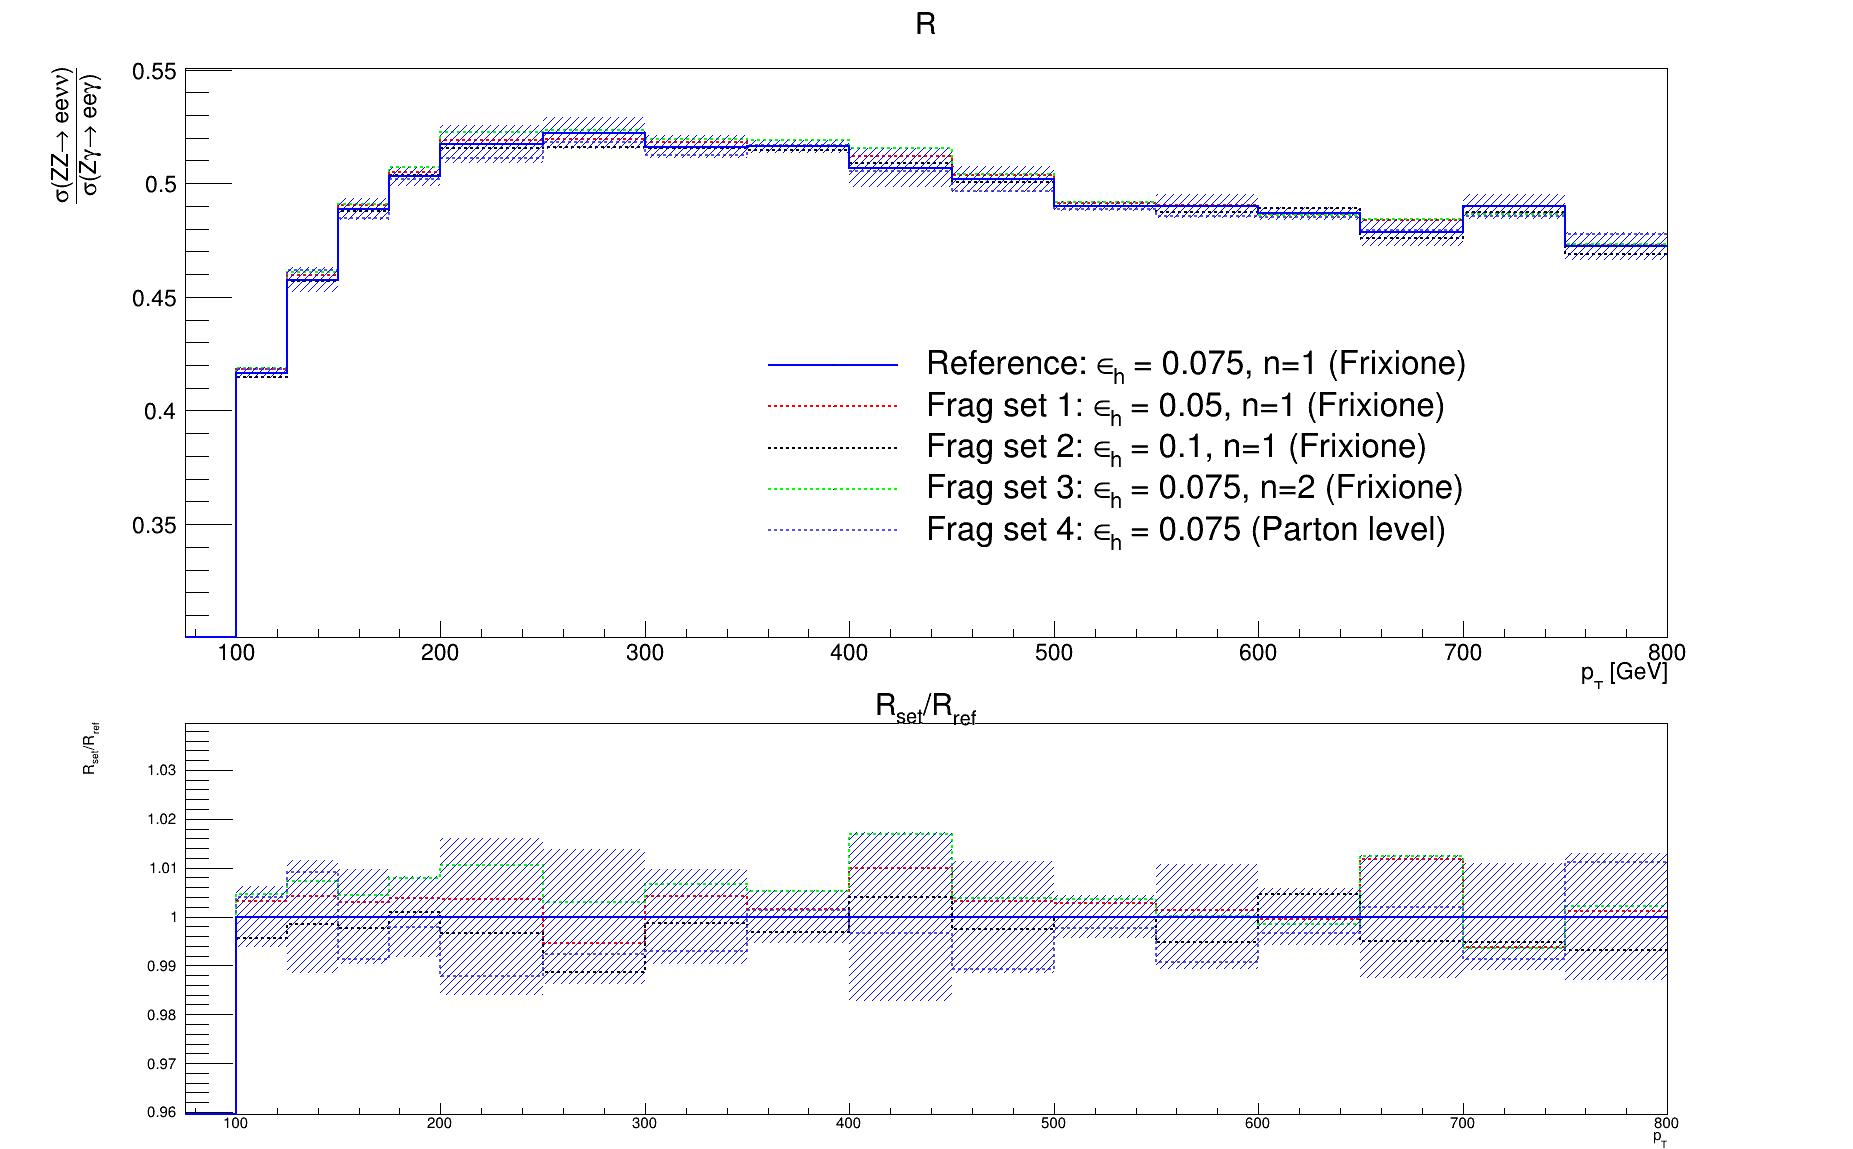
\includegraphics[width=\textwidth]{frag.png}
	\caption{$R$ curve as a function of $p_T$, showing the uncertainty due to variation of photon isolation parameters $\epsilon_h$ and $n$ in the smooth cone isolation procedure (Frixione), and $\epsilon_h$ in the photon isolation procedure. The lower panel shows the relative deviation of the varied sets from the central curve, as well as the uncertainty band.}
	\label{fig:photon_frag}
\end{figure}

The uncertainty is calculated in the following manner:
\begin{equation}
\begin{split}
\delta R_i &= |R_i - R_{ref}| \hspace{2cm}  i \in (1,2,3,4)\\
\delta R &= \sqrt{\max_{i=1,2,3}(\delta R_i)^2 + (\delta R_4)^2}
\end{split}
\end{equation}
as the Frixione procedure and the experimental photon isolation procedure are assumed to be independent.\\
An uncertainty is $< 2\%$ over the whole range, which has been extended up till 800 GeV.

\subsection*{Monte Carlo samples - Truth}
\label{subsec:MC_truth}
\addcontentsline{toc}{subsection}{\nameref{subsec:MC_truth}}
The next step would be to implement the analysis to Monte Carlo samples giving event information at the truth level. For this purpose, $ZZ\rightarrow ll\nu\nu$ and $Z\gamma \rightarrow ll\gamma$ events are generated using POWHEG-PYTHIA\cite{powheg}\cite{pythia}, and run through a detector simulation to obtain an xAOD sample. This sample contains truth level information of the particles.\\
The analysis and comparison to MCFM results has been implemented on the \ZZ process. The cuts on the lepton $p_T$ and $\eta$, as well as the dilepton mass window are as stated in Table \ref{table:default}. For the comparison, only truth level electrons have been considered, for the analysis on the MCFM and the xAOD samples to be as identical as possible.\\
There are some notable differences between the analysis done with MCFM and the xAOD sample.
\begin{itemize}
	\item The xAOD sample is made using a combination of the \texttt{CT10nlo}\cite{CT10} (0-52), \texttt{MSTW2008nlo68cl}\cite{MSTW2008} and \texttt{NNPDF3.0} PDF sets. This corresponds nearly to the \texttt{PDF4LHC15\_nlo} sets in MCFM (which uses CT14nnlo, ).
	\item The xAOD sample consists of contributions from $qq$ and $qg$ processes. The $gg$ process is absent.
\end{itemize}
Thus, an MCFM sample is generated, with the PDF set \texttt{PDF4LHC15\_nlo\_100}, and the \texttt{omitgg} switch turned on in the steering file.

Table \ref{table:xAOD_MCFM_ZZ_compare} shows the comparison of the effective cross section for the \ZZ process\footnote{The analysis and comparison has only been implemented for the \ZZ process for the moment.} as a function of minimum $p_T^{miss}$.

\begin{table}[H]
	\centering
	\begin{tabular}{|c|c|c|}
	\hline
	Min $p_T^{miss}$ [GeV] & MCFM Cross section [fb] & xAOD Cross section [fb]\\
	\hline
	0 & 99.45 $\pm$ 0.8 & 101.17\\
	50 & 49.95 $\pm$ 0.4 & 49.86\\
	100 & 16.86 $\pm$ 0.12 & 15.73\\
	300 & 0.89 $\pm$ 0.008 & 0.69\\
	\hline
	\end{tabular}
	\caption{A comparison of the cross section calculated as per equation \ref{eq:xAOD_xsec_frac} from the xAOD sample, to the cross section obtained from MCFM for the \ZZ process. The contribution from $gg$ process is excluded from both samples}
	\label{table:xAOD_MCFM_ZZ_compare}
\end{table}

The difference between the xAOD sample and the MCFM sample is 1.7\% at low $p_T^{miss}$, but is significantly larger at high $p_T$ due to inadequate statistics. A comparison of the normalized \ZZ $p_T(Z\rightarrow\nu\nu)$ distribution, as shown in Figure \ref{fig:MCFM_xAOD_ZZ_xsec}, displays good agreement in the low $p_T$ region.

\begin{figure}[H]
\centering
	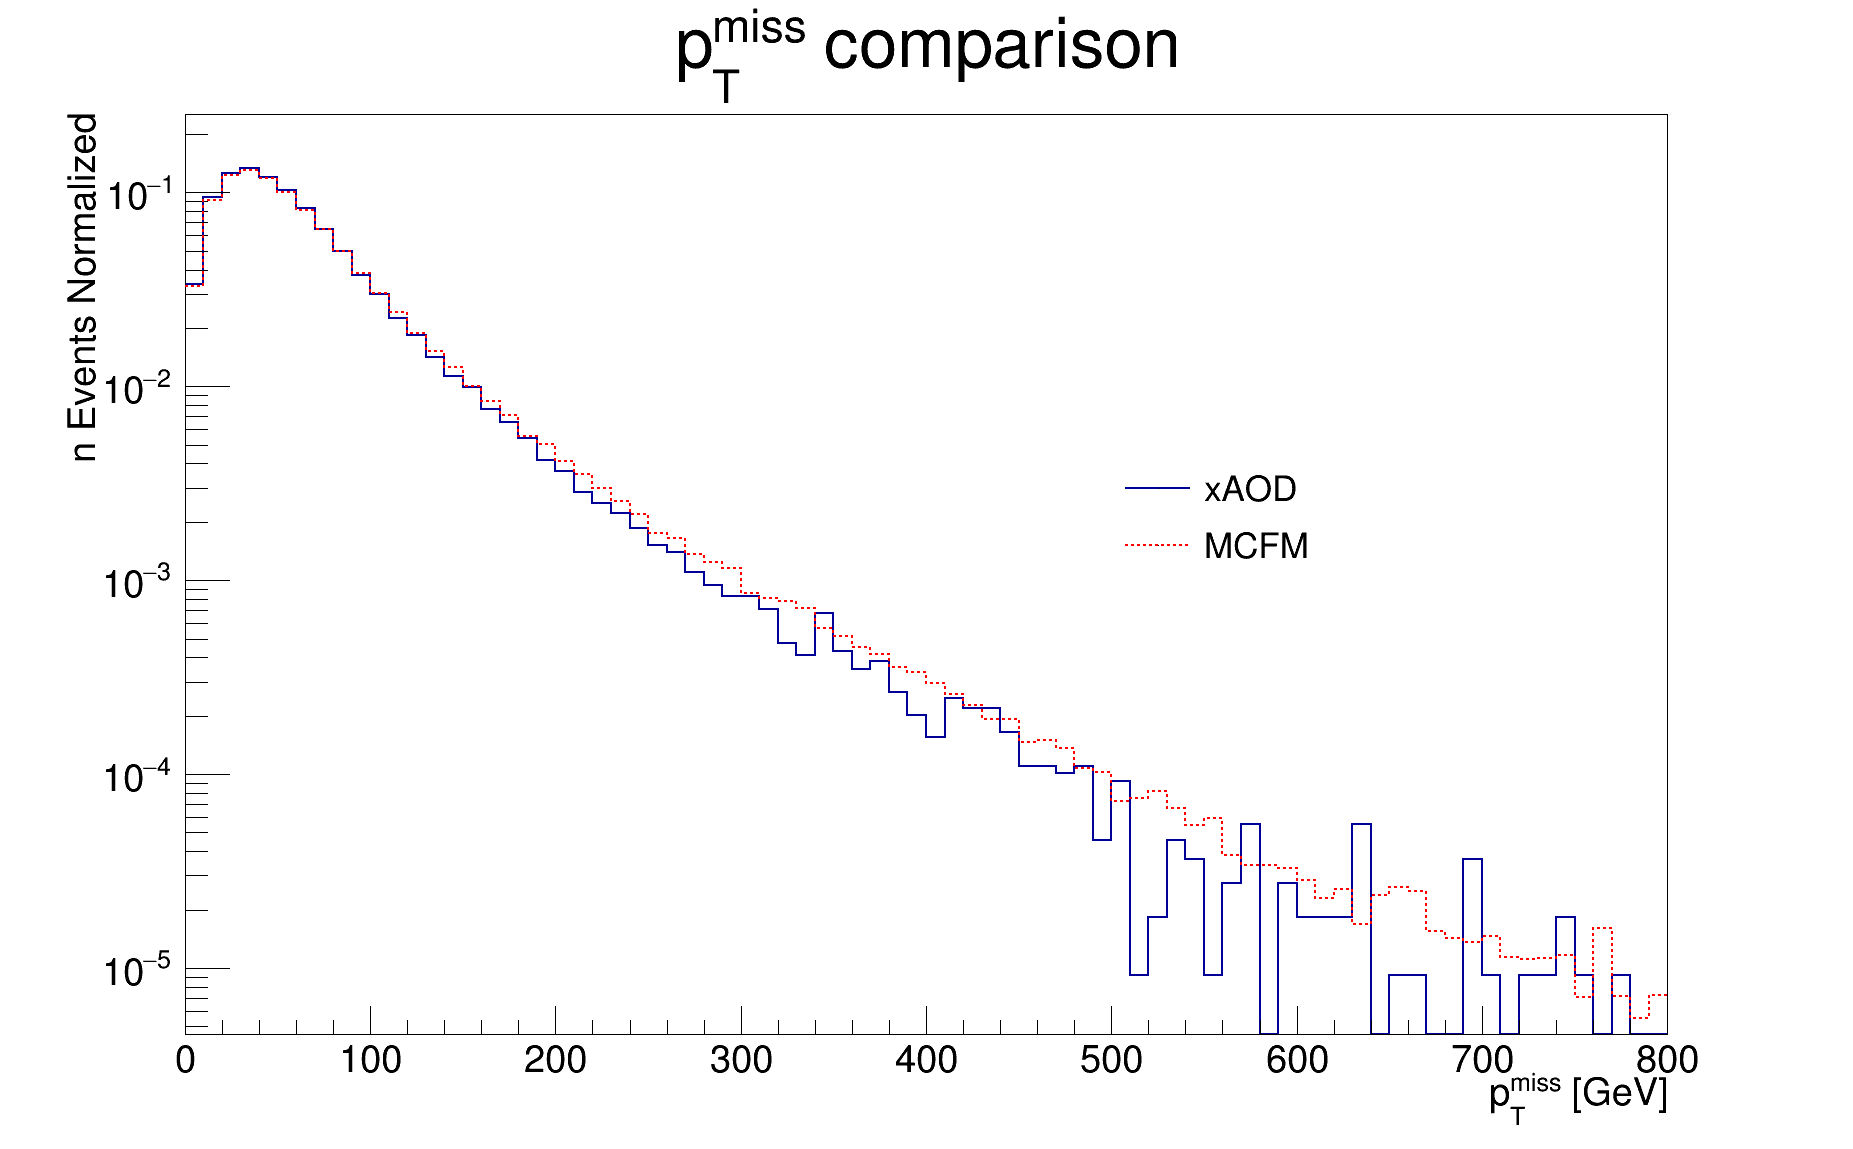
\includegraphics[width=\textwidth]{MCFM_xAOD_ZZ_xsec.png}
	\caption{A comparison of the normalized $p_T(Z\rightarrow\nu\nu)$ spectra from the MCFM and xAOD samples. The shapes agree well in the low $p_T$ region. The high $p_T$ regions suffer from a lack of statistics.}
	\label{fig:MCFM_xAOD_ZZ_xsec}
\end{figure}

\section{Conclusion}
We propose a new method to estimate the \ZZ contribution to the dilepton + MET signal from \Zgam data, using a transfer factor $R$. We quantify the uncertainty from sources such as renormalization and factorization scales and different PDF distributions. From these, we observe that at high $p_T$, the value of $R$ approaches $0.47$. The uncertainty is quantified for $p_T > 100$ GeV slice to be $\approx 2\%$ from scale variation, and $\approx 2.55\%$ from PDF variation, around $R = 0.40$. The uncertainty due to photon fragmentation is $<2\%$ for the full $p_T$ range, up to 800 GeV.

Moving from MCFM cross sections to POWHEG-PYTHIA event samples, we see a good agreement in the low $p_T$ region for the \ZZ process. A deviation of 2\% is observed in this region, which fits within the uncertainty limits obtained thus far. In the high $p_T$ region, better statistics are required.

It remains to observe the effects of $gg$ and $q\bar{q}$ processes separately. Also remaining is to implement the analysis on the \Zgam xAOD samples, to verify agreement, and compare the resulting $R$ curves with the $R$ curves from MCFM.

\section*{Acknowlegements}
This work was conducted under the patient supervision of Dr. Beate Heinemann. In addition to her guidance and advice, I had the help of Dr. Yee Chinn Yapp, who helped me work on streamlining the presentation of this work; Dr. Pieter Everaerts, who helped me debug the code and understand the physics better, and Dr. Sarah Heim, whose office is close enough to mine that I could bother her for the tiniest of details.

\begin{thebibliography}{9}

\bibitem{ZH_ATLAS}
	\textit{Search for an invisibly decaying Higgs boson or dark matter candidates produced in association with a Z boson in pp collisions at $\sqrt{s}$ = 13 TeV with the ATLAS detector}\\
	\textbf{ATLAS Collaboration}\\
	\texttt{arXiv:1708.09624}

\bibitem{gammajet}
	\textit{Using $\gamma +$ jets to calibrate the Standard Model $Z(\rightarrow \nu\nu)+$ jets background to new processes at the LHC}\\
	\textbf{S. Ask, M. A. Parker, T. Sandoval, M. E. Shea, W. J. Stirling}\\
Cavendish Laboratory, University of Cambridge, CB3 0HE, UK; 2011\\
	\texttt{[arXiv:1107.2803]}
	
\bibitem{MCFM}
	\textit{Monte Carlo for FeMtobarn processes (MCFM) v8.0 User Manual}\\
	\textbf{John Campbell, Keith Ellis, Walter Giele, Ciaran Williams}\\
	\texttt{https://mcfm.fnal.gov/}
	
\bibitem{CT14}
	\textit{New parton distribution functions from a global analysis of quantum chromodynamics}\\
	\textbf{Sayipjamal Dulat, Tie Jiun Hou, Jun Gao, Marco Guzzi, Joey Huston, P. Nadolsky, Jon Pumplin, Carl Schmidt, Daniel Stump, C. P. Yuan}\\
	\texttt{arXiv:1506.07443}

\bibitem{PDF4}
	\textit{PDF4LHC recommendations for LHC Run II}\\
	\texttt{[arXiv:1510.03865]}	
	
\bibitem{MMHT14}
	\textit{Parton distributions in the LHC era: MMHT 2014 PDFs}\\
	\textbf{L. A. Harland-Lang, A. D. Martin, P. Motylinski, R. S. Thorne}\\
	\texttt{arXiv:1412.3989}
	
\bibitem{NNPDF3}
	\textit{Parton distributions for the LHC Run II}\\
	\textbf{The NNPDF Collaboration: Richard D. Ball, Valerio Bertone, Stefano Carrazza, Christopher S. Deans, Luigi Del Debbio, Stefano Forte, Alberto Guffanti, Nathan P. Hartland, Jose I. Latorre, Juan Rojo, Maria Ubiali}\\
	\texttt{arXiv:1410.8849}
	
\bibitem{LHAPDF}
	\textit{LHAPDF6: parton density access in the LHC precision era}\\
	\textbf{Andy Buckley, James Ferrando, Stephen Lloyd, Karl Nordstrom, Ben Page, Martin Ruefenacht, Marek Schoenherr, Graeme Watt}\\
	\texttt{arXiv:1412.7420}

\bibitem{frixione}
	\textit{Isolated photons in perturbative QCD}\\	
	\textbf{S. Frixione}\\
	Phys. Lett.B429(1998)369–374, hep-ph/9801442

\bibitem{ATHENA}
	\textit{ATHENA reference}\\
	\texttt{ATHENA reference}
	
\bibitem{powheg}
	POWHEG BOX - ZZ,WZ and WW production
	\begin{itemize}
	\item \textbf{P. Nason}\\
	JHEP 0411 (2004) 040, hep-ph/0409146
	\item \textbf{S. Frixione, P. Nason and C. Oleari}\\
	JHEP 0711 (2007) 070, \texttt{arXiv:0709.2092}
	\item \textbf{S. Alioli, P. Nason, C. Oleari and E. Re}\\
	JHEP 1006 (2010) 043, \texttt{arXiv:1002.2581}
	\item \textit{ZZ, WZ and W+W- production, including Gamma/Z interference, singly resonant contributions and interference for identical leptons}\\
	\textbf{T. Melia, P. Nason, R. Rontsch, G. Zanderighi}\\
	JHEP 1111 (2011) 078, \texttt{arXiv:1107.5051}
	\item \textit{W+W-, WZ and ZZ production in the POWHEG-BOX-V2}\\
	\textbf{P. Nason and G. Zanderighi}\\
	Eur.Phys.J. C74 (2014) 2702, \texttt{arXiv:1311.1365}
	\end{itemize}
	
\bibitem{pythia}
	\textit{PYTHIA 8.1}\\
	\textbf{T. Sjöstrand, S. Mrenna and P. Skands}\\
	JHEP05 (2006) 026, Comput. Phys. Comm. 178 (2008) 852. 
	
\bibitem{CT10}
	\textit{New parton distributions for collider physics}
	\textbf{Hung-Liang Lai, Marco Guzzi, Joey Huston, Zhao Li, Pavel M. Nadolsky, Jon Pumplin, C.-P. Yuan}
	\texttt{arXiv:1007.2241}
	
\bibitem{MSTW2008}
	\textit{Parton distributions for the LHC}\\
	\textbf{A.D. Martin, W.J. Stirling, R.S. Thorne, G. Watt}
	\texttt{arXiv:0901.0002}
	
\end{thebibliography}

\end{document}
